% ***************************** MAIN FILE **********************************

\documentclass[12pt]{scrreprt}           % Art des zu erstellenden Dokuments
% bei zweiseitigem Druck twoside-Option oder book-Klasse verwenden

% ****************************** PREAMBLE **********************************
% **************************** PACKAGE SETUP *******************************
\usepackage[ngerman]{babel}          % Lokalisierung von Typographie, Silbentrennung, etc.

\usepackage{ucs}                     % Erweiterte Unterstützung von UTF-8-Kodierung
% \usepackage[utf8x]{inputenc}       % vor 2021 hilfreiche Unterstützung von UTF-8 in Eingabe-Dateien
                                     % nicht mehr kompatibel mit Texlive 2022
\usepackage[T1]{fontenc}             % Zeichensatzkodierung von LaTeX (Cork-Kodierung)
\usepackage{helvet,courier,mathptmx} % Verwendete Schriftarten

\usepackage[headsepline, plainheadsepline, plainfootsepline] {scrlayer-scrpage}

\usepackage{amsmath}                 % Mathematische Infrastruktur für LaTeX der AMS
\usepackage{amsfonts}                % Mathematische Schriftarten
\usepackage{amssymb}                 % Mathematische Symbole
\usepackage{amsthm}                  % Erweiterung der Theorem-Umgebungen
\usepackage[]{units}					 % für \unit-Befehl
%\usepackage[amssymb]{siunits}		 % für SI-Einheiten (amssymb definiert den Befehl \square des amssymb Packages um. Ist dies nicht gewünscht kann die Option squaren verwendet werden. Dann muss für die SI-Einheiten \squaren anstatt \square verwendet werden.)

%\usepackage{fancyhdr}                % Erweiterte Konfiguration von Kopf/Fußzeile
\usepackage{hyperref}                % Querverweise, Hyperlink, pdf-Konfiguration, etc.

\usepackage{float}                   % Selbstdefinierte Floating-Umbgebungen
\usepackage{tabularx}                % Tabellen mit einstellbarer Spaltenbreite
\usepackage[labelfont=bf]{caption}   % Anpassen der Abbildungs- und Tabellenbeschriftungen

\usepackage{algpseudocode}           % Algorithmen als Pseudocode (basiert auf algorithmicx)
\usepackage{listings}                % Quellcode-Satz (z.B. mit Syntax-Hervorhebung)

\usepackage[pdftex,
%draft							%Figures werden nur als Platzhalter eingeblendet
]{graphicx}						% Erweiterte Unterstützung von Graphiken
\usepackage{textpos}                 % Beliebig platzierte Textboxen
\usepackage{xcolor}                  % TeX-Engine-unabhängige Definition von Farben
\usepackage[printonlyused]{acronym}


\usepackage{pdfpages}

\usepackage[numbers]{natbib}         % Weiter Optionen für die Bibliographie
\usepackage{todonotes}
\usepackage{tabulary}
\usepackage{IEEEtrantools}


% ****************************** TOP MATTER ***********************************
\newcommand{\studenteins}{Mithra Rabet}           % Name
\newcommand{\studentzwei}{}           % Name
\newcommand{\matrNumbereins}{70456621}              % Matrikelnummer
\newcommand{\matrNumberzwei}{}              % Matrikelnummer
\newcommand{\studycourse}{Informatik}           % Studiengang

\newcommand{\supervisor}{Prof. Dr. Ina Schiering} % Betreuer
\newcommand{\institution}{Ostfalia Hochschule} % Hochschule
\newcommand{\subinstitution}{Hochschule Braunschweig/Wolfenbüttel}
\newcommand{\faculty}{Informatik}               % Fachbereich
\newcommand{\toponym}{Wolfenbüttel}                 % Ort

\renewcommand{\subject}{Seminararbeit}  % Art/Thema der Arbeit
\newcommand{\titel}{Praxisbericht: Erstellung eines MVP des IAV Merida Request für Daten- und Analyseanfragen} % Titel der Arbeit
\newcommand{\subtitel}{} % Untertitel
\newcommand{\graduation}{} % Angestrebter Titel (nur bei Abschlussarbeiten, sonst leer lassen/auskommentieren)

\newcommand{\keywords}{{}} % Stichworte (durch Komma getrennt)


% **************************** HYPERREF SETUP *******************************
\definecolor{linkcolor}{rgb}{1,0.5,0}
\hypersetup
{
bookmarks=true,                        % Lesezeichen im PDF erzeugen
bookmarksopen=true,                    % Lesezeichen im PDF sofort anzeigen
backref=true,                          % Rückverweise im Literaturverzeichnis
colorlinks=true,                       % Farbige Verweise
%hidelinks = true,                      % Verweise verbergen (entfernt Farbe und Rahmen)
pdfstartview={FitH},                   % Ansicht des PDFs beim öffnen
pdftitle={\titel},                     % Title des PDFs
pdfauthor={\author , \supervisor},     % Autor des PDFs
pdfsubject={\subject},                 % Thema des PDFs
%pdfcreator={Creator},                 % Erzeuger des Dokuments (Anwendungsprogramm)
%pdfproducer={Producer},               % Ersteller des PDFs (Programm/Bibliothek/Skript)
pdfkeywords={\keywords},               % Stichwörter zum PDF
linkcolor=linkcolor,                   % Farbe von Querverweisen
citecolor=green,                       % Farbe von Zitaten
filecolor=magenta,                     % Farbe von Verweisen auf Dateien
urlcolor=cyan                          % Farbe von URLs
}
% Weitere Optionen: http://www.tug.org/applications/hyperref/manual.html

% **************************** LISTINGS SETUP *******************************
\definecolor{keywords}{rgb}{0.5 0 0.3}
\definecolor{comments}{rgb}{0.25,0.5,0.37}
\lstset{ %
  backgroundcolor=\color{white},   % Hintergrundfarbe
  basicstyle=\linespread{0.94}\footnotesize\ttfamily, % Schrifteinstellungen für Quellcode
  breakatwhitespace=false,         % Automatische Zeilenumbrüche nur bei Leer- oder Tabulatorzeichen (Leerraum/whitespaces)
  breaklines=true,                 % Automatische Zeilenumbrüche
  captionpos=b,                    % Beschriftung unten
  commentstyle=\color{comments},   % Schrifteinstellungen für Kommentare
%  deletekeywords={...},            % Bestimmte Schlüsselwörter entfernen
  escapeinside={\%*}{*)},          % Defintion von Escape-Sequenzen
  extendedchars=true,              % Nicht ASCII-Zeichen erlauben
  frame=single,                    % Rahmen um den Quellcode
  keepspaces=true,                 % Einrückungen im Quellcode behalten
  keywordstyle=\bfseries\color{keywords},% Schrifteinstellungen für Schlüsselwörter
  language=java,                   % Programmiersprache des Quellcodes
%  morekeywords={*,...},            % Zusätzliche Schlüsselwörter
  numbers=left,                    % Zeilennummerierung
  numbersep=5pt,                   % Abstand zwischen Zeilennummerierung und Quellcode
  numberstyle=\tiny\color{gray}, % Schrifteinstellungen für Zeilennummern
  rulecolor=\color{black},         % if not set, the frame-color may be changed on line-breaks within not-black text (e.g. comments (green here))
  showspaces=false,                % Leerraum-Zeichen anzeigen
  showstringspaces=false,          % Leerzeichen in Zeichenketten anzeigen
  showtabs=false,                  % Tabulatorzeichen in Zeichenketten anzeigen
  stepnumber=1,                    % Schrittweite bei Zeilennummern
  stringstyle=\color{blue},        % Schrifteinstellungen für Zeichenketten
  tabsize=4,                       % Tabulatorbreite (Anzahl Leerzeichen)
  numberbychapter=false            % Nummeriere Quellcode fortlaufend je Kapitel
}
\renewcommand{\lstlistlistingname}{Quellcodeverzeichnis}
\renewcommand{\lstlistingname}{Quellcode}

\AtBeginDocument{\numberwithin{lstlisting}{section}} % Nummeriere Quellcode fortlaufend je Abschnitt

% ************************** HEADER/FOOTER SETUP ****************************
\pagestyle{scrheadings}

\clearscrheadings				% löscht voreingestellte Stile
\clearscrplain					% löscht voreingestellte Stile

\lohead[\headmark]{\headmark}
\rohead[\pagemark]{\pagemark}

\automark{chapter}

% **************************** GRAPHICX SETUP *********************************
\DeclareGraphicsExtensions{.pdf,.png,.jpg} % bekannte Graphik-Dateiformate (müssen nicht mehr im Dateinamen angegeben werden, also statt "beispiel.png" nur noch "beispiel")
\graphicspath{{./figure/}}   % path to graphics folder, usage {PATH},{ANOTHERPATH}...

% ************************** BIBLIOGRAPHY SETUP ********************************
\bibliographystyle{IEEEtranN}    % Literaturverzeichnis nach IEEE
%\AtBeginDocument{\nocite{*}} % Diese Zeile vor der Abgabe der Arbeit entfernen!

% ****************************** MATH SETUP ************************************
\everymath{\displaystyle}    % Erzwinge \displaystyle für Mathematischen-Modus


% ************************* THEOREMS AND PROOF *********************************
\newtheoremstyle{thesis}     % Name des neuen Theorem-Stils
{3pt}                        % Abstand oberhalb des Theorems
{3pt}                        % Abstand unterhalb des Theorems
{\itshape}                   % Schrifteinstellungen innerhalb des Theorems
{}                           % Einrückung der Theorem-Überschrift
{\bfseries}                  % Schrifteinstellungen für die Überschrift des Theorems
{}                           % Satzzeichen zwischen Überschrift und Theorem-Rumpf
{\newline}                   % Abstand hinter der Überschrift
{}                           % Spezifikation der Überschrift
  
\theoremstyle{thesis}        % Verwende neuen Theorem-Stil

\newtheorem{theorem}{Satz}[section] % neue Theorem-Umgebung: theorem (Satz)
\providecommand*{\theoremautorefname}{Satz} % autoref-Name für theorem

\newtheorem{definition}{Definition}[section] % neue Theorem-Umgebung: definition (Definition)
\providecommand*{\definitionautorefname}{Definition} % autoref-Name für definition

\renewcommand{\qedsymbol}{$\blacksquare$} % Schwarzes Quardrat als Symbol für: q. e. d.
\renewenvironment{proof}[1][\proofname]{{\bfseries #1:}~}{\qed} % "Beweise:" in Fettdruck

% *************************** PSEUDOCODE SETUP ********************************
\floatstyle{boxed}                        % Rahmen für pseudocode-Umgebung
\newfloat{pseudocode}{htbp}{lop}[section] % Definieren pseudocode-Umgebung
\floatname{pseudocode}{Pseudocode}        % Beschrifte pseudocode-Umgebung mit "Pseudocode"

\newcommand{\listofpseudocodename}{Pseudocodeverzeichnis}
\newcommand{\listofpseudocode}{\listof{pseudocode}{\listofpseudocodename}}
\providecommand*{\pseudocodeautorefname}{Pseudocode}

% ******************************* PAGE SETUP **********************************
\textheight23cm
\textwidth14cm
\voffset0cm
\topskip0cm
\topmargin-1.2cm
\headheight1.0cm
\headsep1.5cm
\oddsidemargin1.0cm
\evensidemargin1.0cm
\renewcommand{\baselinestretch}{1.4} 
%\parindent0pt

% Hurenkinder und Schusterjungen verhindern
\clubpenalty = 10000
\widowpenalty = 10000
\displaywidowpenalty = 10000

% Verbesserung der Textsetzung
\tolerance = 1000
\emergencystretch = 20pt

% ******************************** MACROS *************************************
\newcommand{\RR}{\mathbf{R}}
\newcommand{\NN}{\mathbf{N}}
\newcommand{\QQ}{\mathbf{Q}}
\newcommand{\ZZ}{\mathbf{Z}}
\newcommand{\CC}{\mathbf{C}}
\newcommand{\erstelltvon}[1]{\marginpar{\fbox{#1}}}


% ************************** DOCUMENT **************************************
\begin{document}
\bstctlcite{IEEEexample:BSTcontrol} 
\pagestyle{plain}

% 
%% *** Titelseite ***
%
\begin{titlepage}
	%\centering
	\vspace*{-3.0cm}
	%Logo international
	%\hspace*{ 9.30cm}
\includegraphics[scale=0.93]{../ostfalia/LSVorlagejpg_klein_int.jpg}\\
	%Logo deutsch
	%\hspace*{10.20cm}
\includegraphics[scale=0.60]{../ostfalia/Ostfalia_LS_RGB_klein.jpg}\\
	\hspace*{ 6.90cm}
\includegraphics[scale=0.93]{ostfalia/Ostfalia_LS_RGB_klein.jpg}\\
	%Logo ohne Schrift
	%\hspace*{15.00cm}
\includegraphics[scale=0.60]{../ostfalia/Ostfalia_L_RGB_klein.jpg}\\
	%\hspace*{14.30cm}
\includegraphics[scale=0.93]{../ostfalia/Ostfalia_L_RGB_klein.jpg}\\
	\hspace*{-1.00cm}
\includegraphics[scale=1.20]{ostfalia/Reiter_Wolfen_RGB_174mm.jpg}\\
	
	\hspace*{-0.5cm}{\Large\textsf{Fakultät \faculty}}\\
	
	\hrulefill\\
	
	%-------------------------------------------------------------------------------
	\noindent{\Large\textsf{\studenteins, \matrNumbereins\\}}
	\ifdefined\studentzwei%
	\if\studentzwei\empty
	\else
	{\Large\textsf{\studentzwei, \matrNumberzwei\\}}
	\fi
	
	
	\vspace{2em}
	\begin{center}
		
		\textbf{
			\textsf{\huge\titel \\[0.3ex]}}
		\end{center}
	% \textsf{\hspace*{0.5cm}\large \subtitel \\[0.05cm]}
	
	\vspace{2em}
	\begin{center}
	\ifdefined\graduation%
	\if\graduation\empty%
	\else%
	\textsf{Abschlussarbeit zur Erlangung des akademischen Grades}\\[0.5cm]
	\textsf{\graduation} \textsf{im Studiengang Informatik}\\[0.5cm]
	\textsf{an der \institution}\\[0.5cm]
	\textsf{\subinstitution}
	\fi
	\end{center}
	
	\vspace*{\fill}

 	\enlargethispage{1\baselineskip}
	\hrulefill\\
	\begin{center}
		\textsf{Betreuerin: \\  \supervisor}
	\end{center}
	
	\vspace*{\fill}
	
	%-------------------------------------------------------------------------------
	
	\enlargethispage{4\baselineskip}
	\begin{minipage}[b]{0mm}
		\raisebox{24mm}{\hspace*{-1.00cm}
\includegraphics[scale=1.20]{ostfalia/Reiter_szsudwob_RGB_174mm.jpg}}
	\end{minipage}
	
	%*******************************************************************************
	
\end{titlepage}


% ***************************** FRONT MATTER *******************************
\setcounter{page}{1}
\pagenumbering{Roman}
\section*{Erklärung}
\vspace*{0.5cm}
\noindent
Hiermit versichere ich, dass ich die vorliegende Arbeit selbstständig verfasst und keine anderen als die angegebenen Quellen und Hilfsmittel benutzt habe. Ich versichere, dass ich alle wörtlich oder sinngemäß aus anderen Werken übernommenen Aussagen als solche gekennzeichnet habe. Dies gilt explizit auch für die Verwendung von text- oder codegenerierenden KI-Werkzeugen.

Die eingereichte Arbeit ist weder vollständig noch in wesentlichen Teilen Gegenstand eines anderen Prüfungsverfahrens gewesen.

Ich habe zur Kenntnis genommen, dass die Arbeit einer elektronischen Plagiatsprüfung unterzogen werden kann.

\vspace{3cm}
\toponym, den \today
%\chapter*{Überblick}
\section*{Kurzfassung}
Hier sollte eine halbseitige Kurzfassung der Arbeit stehen.
\vfill\vfill\vfill\vfill\vfill\vfill
\section*{Abstract}
Here, an abstract written in English should appear.
\vfill\vfill\vfill\vfill\vfill\vfill
% *************************** TABLE OF CONTENTS *******************************
% ************************* (Inhaltsverzeichnis) ******************************
% Die Auskommentierte Zeile fügt das Inhaltsverzeichnis zum Inhaltsverzeichnis hinzu. Diese Verhalten kann auch über das Paket tocbibind erreicht werden. Allerdings funktioniert das Paket nicht für das Pseudocodeverzeichnis, aus diesem Grund werden die Einträge "manuell" hinzugefügt.

%\phantomsection\addcontentsline{toc}{chapter}{\numberline{}\contentsname}
{
\baselineskip=15pt % Schriftlinien-Abstand 15 pt (nur beim Inhaltsverzeichnis)
\tableofcontents   % Inhaltsverzeichnis einfügen
}
{
\baselineskip=22pt % Schriftlinien-Abstand 22 pt (bei allen anderen Verzeichnissen)

% **************************** LIST OF FIGURES ********************************
% ************************ (Abbildungsverzeichnis) ****************************
\clearpage\phantomsection
%\addcontentsline{toc}{chapter}{\numberline{}\listfigurename}

\listoffigures % Abbildungsverzeichnis einfügen

% **************************** LIST OF TABLES *********************************
%\clearpage\phantomsection\addcontentsline{toc}{chapter}{\numberline{}\listtablename}

%\listoftables % Tabellenverzeichnis einfügen

% ************************** LIST OF PSEUDOCODE *******************************
%\clearpage\phantomsection\addcontentsline{toc}{chapter}{\numberline{}\listofpseudocodename}

%\listofpseudocode % Pseudocodeverzeichnis einfügen

% *************************** LIST OF LISTINGS ********************************
%\clearpage\phantomsection\addcontentsline{toc}{chapter}{\numberline{}\lstlistlistingname}

%\lstlistoflistings % Quellcodeverzeichnis einfügen
}
\addchap{Abkürzungsverzeichnis}
\begin{acronym}[long]
	\acro{CPIC}{Customer and Product Intelligence Center}
	\acro{CI/CD}{Corperate Identity/Corporate Design}
	\acro{MVC}{Model-View-Controller}
	\acro{ORM}{Object-Relational Mapping}
\end{acronym}


% ***************************** MAIN MATTER ********************************
\pagenumbering{arabic}

\chapter{Einleitung}
\label{chap:einleitung}
\erstelltvon{student 1}
Worum geht is in Ihrer Arbeit?

\section{Motivation}
\label{sec:motivation}
Was ist die Motivation hinter dieser Arbeit?

\section{Zielsetzung}
\label{sec:zielsetzung}
Ziele der Arbeit.

\section{Aufbau}
\label{sec:aufbau}
Aufbau der Arbeit. Sehr kurz. Abkürzungen führt man übrigens mit \acfi{acfi} ein.


\chapter{Hintergrund und Ziele des Projekts}
\label{chap:grundlagen}
Das vorliegende Projekt beschäftigt sich mit der Anpassung und Erweiterung eines bestehenden Tools, um es den spezifischen Anforderungen der IAV GmbH gerecht zu machen. Zur Verbesserung interner Prozesse und Abläufe in der Messdatenverwaltung möchte IAV die Idee des für BMW entwickelten RequestChannels adaptieren und mit den gesammelten Erfahrungen für die eigenen Anforderungen umsetzen.
\newline
Um dieses Ziel zu erreichen, müssen spezifische Anforderungen im Hinblick auf das Design, die Funktionalitäten und die nahtlose Integration in die bestehende Infrastruktur berücksichtigt werden. 
\newline
Die folgenden Abschnitte erläutern detailliert die Ziele des Projekts sowie die strategischen und technischen Hintergründe, die dieses Vorhaben leiten.
\section{Hintergrund des Projekts}
Der Hintergrund dieses Projekts liegt in der wachsenden Bedeutung der Digitalisierung. In den letzten Jahren sind zahlreiche Herausforderungen in Bezug auf den Zugang und die Nutzung von Daten aufgetreten. Insbesondere der EU Data Act, der am 11. Januar 2024 in Kraft trat, schafft einen neuen Rechtsrahmen, der den fairen und transparenten Zugang zu Daten sowie deren Nutzung regeln soll. Dies soll vor allem dazu beitragen, die Dominanz großer, globaler Tech-Konzerne im Bereich Datenspeicherung und -verarbeitung zu verringern und einen ausgewogeneren Wettbewerb zu ermöglichen .\cite{EUData_JohnerInstitut,bmdv2024}
\newline
Mittels des EU Data Acts soll ein fairer Wettbewerb geschaffen werden, da aktuell die Dominanz der US-Techkonzerne in Bezug auf Datenspeicherund und -verarbeitung diesen gefährden. \cite{EUData_JohnerInstitut}
\newline
Auch IAV ist direkt vom EU Data Act betroffen und benötigt ein spezifisches Tool, um externe Anfragen nach Daten regelkonform bearbeiten zu können. Dies betrifft insbesondere die gesetzlich vorgeschriebenen Anforderungen an den Datenaustausch und die Transparenz der Nutzung, wie sie im EU Data Act festgelegt sind.
\newline
Neben dem externen Bedarf durch den EU Data Act ist der IAV Merida Request jedoch auch von entscheidender Bedeutung für interne Abläufe bei IAV. Der IAV Merida Request soll einen Kanal etablieren, der Kunden und IAV-Mitarbeitern einen effizienten und strukturierten Workflow ermöglicht.
\newline
\newline
Im Rahmen dieses Studentenprojekts wird eine Whitelabel-Version des BMW RequestChannel entwickelt. Diese Plattform dient BMW als zentrale Anlaufstelle für Analyseanfragen und könnte in ähnlicher Weise für IAV als Datenmanagement- und Anfragetool eingesetzt werden. Die Whitelabel-Version soll als flexible und anpassbare Lösung entwickelt werden, die sowohl interne als auch externe Anforderungen erfüllt.
\newline
Der BMW RequestChannel ist Teil des BMW \ac{CPIC} und ermöglicht es, neue Analyseanfragen zu verschiedenen Datenquellen zu stellen, wenn keine bestehenden Auswertungen über die \ac{CPIC}-Kanäle verfügbar sind. Auf ähnliche Weise soll der IAV Merida Request nicht nur intern genutzt werden, sondern später auch den Anforderungen des EU Data Act gerecht werden, indem es Anfragen von Dritten entsprechend verwaltet und bearbeitet. 
\newline
Die verschiedenen Use Cases, die mögliche Einsatzszenarien des Tools beschreiben, wurden ausgearbeitet und werden im späteren Verlauf des Berichts näher erläutert. Im Rahmen dieses Studentenprojekts liegt der Schwerpunkt jedoch auf dem ersten Use Case, „Projektinterne Anfragen über den IAV Merida Projektexplorer“. Dieser wird detailliert beschrieben und dient als Grundlage für die technische Implementierung.
\section{Ziele des Projekts}
Das Hauptziel des Projekts besteht darin, das bestehende BMW RequestChannel-Tool durch Whitelabeling an die spezifischen Anforderungen und das Branding der IAV GmbH anzupassen. Whitelabeling bedeutet in diesem Kontext, das Tool so zu modifizieren, dass es optisch, funktional und markentechnisch in die IAV-Umgebung integriert wird. Dies umfasst Änderungen am Benutzerinterface, um es mit den \ac{CI/CD} von IAV anzupassen. Neben der visuellen Anpassung ist es auch notwendig, sicherzustellen, dass die Software den spezifischen technischen und funktionalen Bedürfnissen von IAV entspricht. Dies könnte etwa spezielle Workflows oder Zugriffsrechte beinhalten, die für IAV-Nutzer relevant sind.
\newline
\newline
Ein weiteres zentrales Ziel des Projekts ist die reibungslose Integration des angepassten RequestChannel-Tools in die bestehende IAV Merida Toolkette. Die IAV Merida Toolkette bietet eine Infrastruktur für die Nutzung und Verwaltung von Messdaten sowie für Analysen und andere Entwicklungsprozesse. Es ist entscheidend, dass das Tool nahtlos in diese Umgebung eingebettet wird, damit Benutzer direkt auf das Tool zugreifen und es effizient in ihre bestehenden Arbeitsprozesse integrieren können. Dies umfasst die Integration der Kommunikationsschnittstellen, die Datenübertragung zwischen den verschiedenen Tools sowie die Sicherstellung, dass das RequestChannel-Tool innerhalb der Merida-Plattform stabil und zuverlässig läuft. Durch diese Integration wird der Workflow zur Bereitstellung von Daten- und Analysen optimiert. 
\newline
\newline
Zudem müssen die vorher definierten Use Cases, die eine Erweiterung der Nutzungsmöglichkeiten des Tools beschreiben, implementiert werden. Diese Use Cases sind oft auf spezielle Arbeitsprozesse, Bedürfnisse oder Herausforderungen innerhalb von IAV zugeschnitten. Die Erweiterung der Funktionalitäten kann beispielsweise die Implementierung zusätzlicher Automatisierungsfunktionen, Berichts- und Analyseoptionen oder die Integration neuer Schnittstellen betreffen. 
\newline
Im Rahmen des Projekts liegt der Fokus auf der Umsetzung des ersten Use Cases. Ziel ist es, eine zentrale Plattform zu schaffen, die Kundenanfragen über den IAV Merida Projektexplorer effizient verwaltet und die Bearbeitung dieser Anfragen verbessert. Weitere Use Cases werden im Hinblick auf eine potenzielle zukünftige Erweiterung betrachtet, jedoch nicht im aktuellen Projekt implementiert.
\newline
Das Ziel ist es, das Tool so zu optimieren, dass es für die IAV-Anwender nicht nur die vorhandenen Anforderungen erfüllt, sondern auch zusätzliche Mehrwerte bietet. Dadurch wird das Tool zu einer flexiblen Lösung, die in verschiedenen Anwendungsbereichen effizient eingesetzt werden kann. Es soll die Möglichkeit bieten, unterschiedliche Arbeitsprozesse zu unterstützen und nahtlos in verschiedene Szenarien integriert zu werden, um den Mehrwert für IAV-Anwender in vielfältigen Einsatzgebieten zu maximieren.
\label{chap:kapitel2}



%\chapter{Grundlagen? Außerhalb des Allgemeinwissens Informatik}
\label{chap:kapitel3}

\chapter{Anforderungen des Projekts}

Im Rahmen des Projekts wurden drei zentrale Use Cases herausgearbeitet, die die verschiedenen Anwendungsszenarien des modifizierten RequestChannel-Tools beschreiben. Jeder Use Case adressiert spezifische Anforderungen und Anwendungsfälle, die für die IAV-Nutzer von hoher Relevanz sind. Die erfolgreiche Implementierung dieser Use Cases erweitert die Funktionalität des Tools und optimiert die Arbeitsabläufe bei der Anfrage und Analyse von Messdaten.
\section{Anfragen externer Messdaten und Analysen im Rahmen des EU-DataActs}
Dieser Use Case beschreibt die Möglichkeit, dass ein Drittanbieter Zugriff auf die Betriebsdaten eines Fahrzeugs erhält, das von einem Kunden betrieben oder getestet wird. Dies geschieht im Rahmen des EU-DataActs, der den Austausch und die Bereitstellung von Daten zwischen Unternehmen fördert. Der EU Data Act spielt dabei eine entscheidende Rolle, da er sicherstellt, dass der Kunde das alleinige Recht über die Nutzung und Weitergabe der generierten Fahrzeugdaten besitzt.  \cite{bmdv2024} Dies bedeutet, dass der Kunde entscheiden kann, ob und in welchem Umfang er diese Daten an externe Dienstleister weitergeben möchte.
\newline
Der Prozess beginnt mit der kontinuierlichen Generierung von Betriebsdaten durch das Fahrzeug. Diese Daten umfassen verschiedene Aspekte des Fahrzeugbetriebs, wie Leistungskennzahlen, Kraftstoffverbrauch, Abnutzung und weitere für den Drittanbieter relevante Informationen. Die erfassten Daten werden in der IAV-internen Merida-Infrastruktur gespeichert und verwaltet, sodass sie jederzeit abrufbereit sind.
\newline
Wenn ein Drittanbieter Interesse an diesen Daten hat, stellt er eine offizielle Anfrage an den Kunden. Diese Anfrage betrifft spezifische Betriebsdaten, die für die Weiterentwicklung von Dienstleistungen oder Analysen des Drittanbieters von Nutzen sein könnten. Hier tritt der EU Data Act in Kraft, indem er sicherstellt, dass der Kunde in der Position ist, vollständig über die Verwendung seiner Daten zu entscheiden. Das gibt dem Kunden die volle Kontrolle über den weiteren Prozess.
\newline
\newline
Nach der Anfrage folgt in der Regel eine Phase der Vertragsverhandlung, in der der Kunde und der Drittanbieter die Bedingungen für den Datenzugriff klären. Dabei geht es unter anderem um Fragen wie die Art der Daten, die freigegeben werden sollen, die Dauer des Datenzugriffs und mögliche Vergütungsregelungen. Der EU Data Act sorgt dafür, dass diese Verhandlungen fair und transparent ablaufen, sodass der Kunde jederzeit die Entscheidungsgewalt behält.
\newline
Sobald die Vertragsbedingungen festgelegt sind, entscheidet der Kunde, welche spezifischen Daten an den Drittanbieter übermittelt werden. Der Drittanbieter hat dann die Möglichkeit über das IAV Merida Request-Tool die gespeicherte Daten oder Analysen anzufragen. Es wird sichergestellt, dass diese Freigabe unter Berücksichtigung der Datenschutzbestimmungen erfolgt und dass nur die vereinbarten Daten bereitgestellt werden.
\newline
Nachdem die Daten oder Analysen an den Drittanbieter übermittelt wurden, kann dieser mit der Nutzung beginnen. Die gewonnenen Erkenntnisse könnten beispielsweise in die Entwicklung neuer Produkte oder Dienstleistungen einfließen, wobei der gesamte Prozess durch die klare Regelung des EU Data Acts strukturiert und kontrolliert wird.
\newline
Das folgende Diagramm bildet den beschriebenen Use Case ab und veranschaulicht die Interaktionen innerhalb des Prozesses von der Datengenerierung bis zur Speicherung. Zudem werden die Abhängigkeiten zwischen diesen Schritten deutlich gemacht.
\begin{figure}[H]
    \centering
    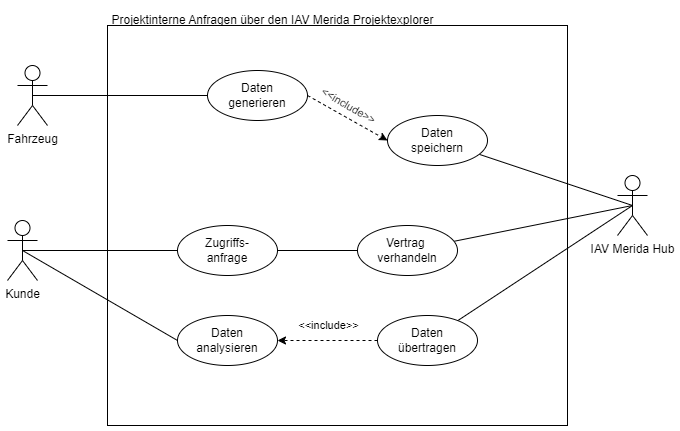
\includegraphics[scale=.6]{media/UseCase1}
    \caption{UseCase1}
    \label{fig:UseCase1}
\end{figure}
\newpage
\section{Projektinterne Anfragen über den IAV Merida Projektexplorer}
Ein weiterer wichtiger Use Case betrifft die projektinternen Anfragen von Messdaten und Analysen durch IAV-Mitarbeiter. Über das Merida Request-Tool haben die Mitarbeiter die Möglichkeit, Daten, die für bestimmte Projekte relevant sind, anzufragen. Dieser Anwendungsfall unterstützt die Optimierung der internen Arbeitsabläufe und verbessert den Zugriff auf projektbezogene Informationen, die für die Entwicklung und Analyse von großer Bedeutung sind.
\newline
Der Merida Hub dient als eine Plattform, über die Mitarbeiter spezifische Messdaten anfordern können. Hierbei handelt es sich vor allem um interne Daten, die während der laufenden Projekte generiert wurden. Diese Daten sind häufig in den IAV-internen Systemen gespeichert und können von den Projektmitgliedern angefragt werden, um fundierte Entscheidungen im Entwicklungsprozess zu treffen. Der Anforderungsprozess über das Merida Request-Tool ermöglicht es den Nutzern, gezielt nach relevanten Daten zu suchen oder sich Analysen erstellen zu lassen und diese in einem einheitlichen Format zu erhalten, was die weitere Bearbeitung erleichtert.
\newline
Auch in diesem Szenario ist es wichtig, dass die Anfrage vor der Bereitstellung der Daten aus finanzieller Sicht geprüft wird. Ein IAV-Mitarbeiter muss sicherstellen, dass die Datenanfrage aus Kostensicht gerechtfertigt ist und keine unnötigen Kosten für das Unternehmen entstehen. Hierbei wird insbesondere der Umfang der angeforderten Daten sowie die potenziellen finanziellen Auswirkungen der Anfrage bewertet. Diese Prüfung stellt sicher, dass die Datenanfragen effizient und im Rahmen des vorgegebenen Budgets bearbeitet werden können.
\newline
Sobald die finanzielle Prüfung abgeschlossen und die Anfrage genehmigt ist, werden die angefragten Daten sicher und kontrolliert an den IAV-Mitarbeiter übertragen. Über den Merida Hub kann der IAV-Mitarbeiter dann auf die freigegebenen Daten oder Analysen zugreifen und diese für sein Projekt nutzen. Die Sicherheit der Datenübertragung spielt dabei eine wesentliche Rolle, um sicherzustellen, dass alle sensiblen Informationen geschützt bleiben und nur autorisierte Personen Zugriff erhalten.
\newline
Der IAV-Mitarbeiter verwendet die übermittelten Daten oder Analysen anschließend zur Untersuchung der Fahrzeugleistung und -zuverlässigkeit. Dies ermöglicht es ihm, gezielte Optimierungen an seinen Produkten vorzunehmen, was wiederum zur Verbesserung der Produktqualität und zur Effizienzsteigerung führt.
\newline
In dem folgendem Diagramm veranschaulicht den Use Case für die Anfrage von IAV-Mitarbeitern.
\begin{figure}[H]
    \centering
    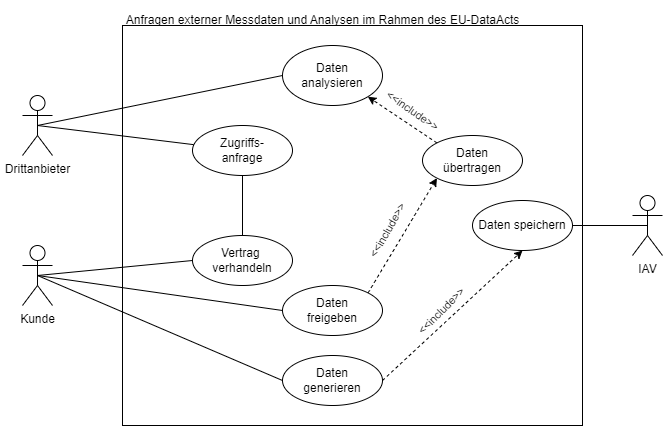
\includegraphics[scale=.6]{media/UseCase2}
    \caption{UseCase2}
    \label{fig:UseCase2}
  \end{figure}
  \newpage
\section{Anfragen von Daten eines Dritten und Bezahlung über Mobilfunkbetreiber}
Dieser Use Case beschreibt einen Prozess, bei dem Fahrzeugführer ihre Betriebsdaten monetarisieren können, indem sie diese an interessierte Parteien wie Versicherungsunternehmen oder OEMs verkaufen. Die dabei verwendeten Daten können von großem Nutzen für Unternehmen sein, die wertvolle Einblicke in die Fahrzeugnutzung gewinnen wollen, um ihre eigenen Produkte oder Dienstleistungen zu optimieren. Gleichzeitig ermöglicht dieser Prozess dem Fahrzeugführer, von den generierten Daten finanziell zu profitieren.
\newline
Auch hier werden die Fahrzeugdaten kontinuierlich erfasst und im Merida Hub gespeichert. Versicherungsunternehmen oder OEMs, die an diesen Daten interessiert sind, stellen eine Anfrage an den Fahrzeugführer über einen Daten-Sammel- und Verteilungsdienst, der die gesamte Abwicklung steuert. Diese interessierten Parteien sind insbesondere an den Nutzungsdaten des Fahrzeugs interessiert, um bessere Risikoanalysen durchzuführen oder spezifische Produkte für bestimmte Fahrzeugtypen zu entwickeln.
\newline
\newline
Nach der Anfrage folgt eine Phase der Vertragsverhandlung, in der die Bedingungen für den Datenzugriff geklärt werden. Der Fahrzeugführer, der als Datenverkäufer agiert, hat dabei die Möglichkeit, die Konditionen auszuhandeln und den Preis für die Bereitstellung seiner Daten festzulegen. Ziel ist es, eine faire und ausgewogene Vereinbarung zu treffen, die sowohl den Interessen des Fahrzeugführers als auch denen der interessierten Parteien gerecht wird.
\newline
Die Datenübertragung erfolgt sicher und kontrolliert über das 5G-Netzwerk eines Netzbetreibers wie Telefónica. Dieser Mobilfunkbetreiber spielt eine zentrale Rolle, indem er nicht nur die Datenübertragung gewährleistet, sondern auch die Zahlungstransaktionen abwickelt. Dies sorgt für eine reibungslose und schnelle Bereitstellung der Daten sowie eine unkomplizierte Bezahlung des Fahrzeugführers.
\newline
Die interessierten Parteien nutzen die erhaltenen Daten anschließend, um ihre Produkte und Dienstleistungen zu verbessern. Beispielsweise könnten Versicherungsunternehmen anhand der Fahrzeugnutzungsdaten maßgeschneiderte Versicherungspakete anbieten, die auf das individuelle Fahrverhalten des Fahrzeugführers zugeschnitten sind. OEMs hingegen könnten die Daten verwenden, um die Leistung ihrer Fahrzeuge besser zu verstehen und zukünftige Modelle zu optimieren.
\newline
Dieser Use Case bietet somit allen beteiligten Akteuren Vorteile: Der Fahrzeugführer profitiert finanziell von seinen Daten, während die interessierten Unternehmen wertvolle Einblicke gewinnen, um ihre Geschäftsprozesse und Angebote zu verbessern.
\newline
Das nachstehende Diagramm veranschaulicht den Use Case für die Anfrage von Daten eines Dritten sowie die Bezahlung über einen Mobilfunkanbieter.
\begin{figure}[H]
    \centering
    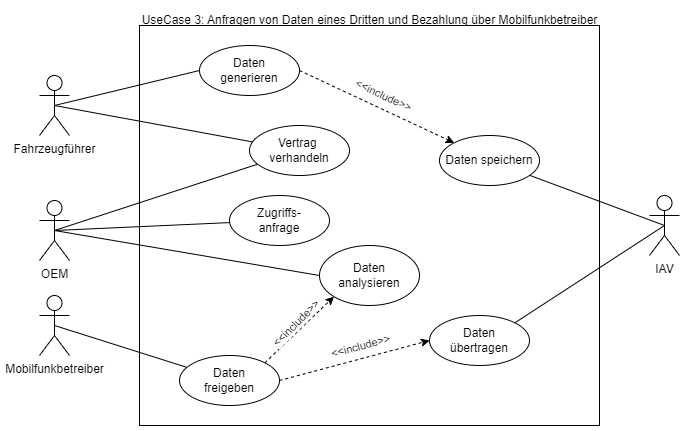
\includegraphics[scale=.6]{media/UseCase3}
    \caption{UseCase3}
    \label{fig:UseCase3}
  \end{figure}
\label{chap:kapitel4}


\chapter{Konzeption}
In diesem Kapitel wird der konzeptionelle Entwurf der entwickelten Lösung detailliert beschrieben. Die Konzeption umfasst alle wesentlichen Aspekte der Benutzeroberfläche, der Prozessabläufe sowie der Systemarchitektur. Dabei war es entscheidend, sowohl die technischen Anforderungen als auch die Nutzerbedürfnisse optimal zu berücksichtigen.
\newline
Zunächst werden die Mockups vorgestellt, die die geplanten Benutzeroberflächen visualisieren. Diese grafischen Entwürfe dienen als Grundlage für die spätere Implementierung der Benutzeroberfläche und helfen dabei, die Nutzerinteraktionen und das Design bereits in der frühen Phase des Projekts zu planen.
\newline
Daraufhin wird der Workflow des Anfrageprozesses dargestellt, um die Abfolge und Logik der einzelnen Prozessschritte zu veranschaulichen. Dies bildet die Grundlage für die spätere Implementierung der Abläufe und dient dazu, alle Beteiligten über die genauen Prozessschritte zu informieren.
\newline
Abschließend wird die Systemarchitektur präsentiert, die das fundamentale Gerüst der gesamten Anwendung bildet. Die Architektur beschreibt die wichtigsten Komponenten und deren Interaktionen, um eine stabile, skalierbare und erweiterbare Lösung zu gewährleisten.
\newpage
\section{Mockups}
Im Verlauf der Entwicklung des IAV Merida Request wurden regelmäßig Gespräche mit verschiedenen Stakeholdern geführt. Diese Interaktionen führten zur schrittweisen Anpassung der Mockups, die auf den gewonnenen Erkenntnissen basierten. Dadurch konnten die Mockups kontinuierlich an die sich entwickelnden Anforderungen und das gewünschte User Interface angepasst werden. Im Folgenden wird der Entwicklungsprozess der Mockups sowie deren verschiedene Versionen detailliert dargestellt.
\subsection*{Mockup 1}
In der ersten Version der Mockups, s. Abbildung \ref{fig:MockUps1.0}, orientierten sich die Designentscheidungen stark am BMW Request Channel. Die Struktur und die Benutzeroberfläche in dieser Phase waren relativ einfach gehalten, mit einem klaren Fokus auf die wesentlichen Eingabefelder und -optionen, die für das Anfordern von Daten und Analysen benötigt wurden.
\newline
Wichtige Merkmale dieser Version:
\begin{itemize}
    \item Eine klare und strukturierte Eingabe für persönliche Details, Datenanforderungen und den gewünschten Ausgabetyp (z.B. „Raw Data“ oder „Analysis“).
    \item Es wurde darauf geachtet, dass die Navigation zwischen den Schritten unkompliziert und intuitiv ist, allerdings war das Design noch stark an dem Layout des BMW Request Channel angelehnt.
\end{itemize}
\begin{figure}[H]
    \centering
    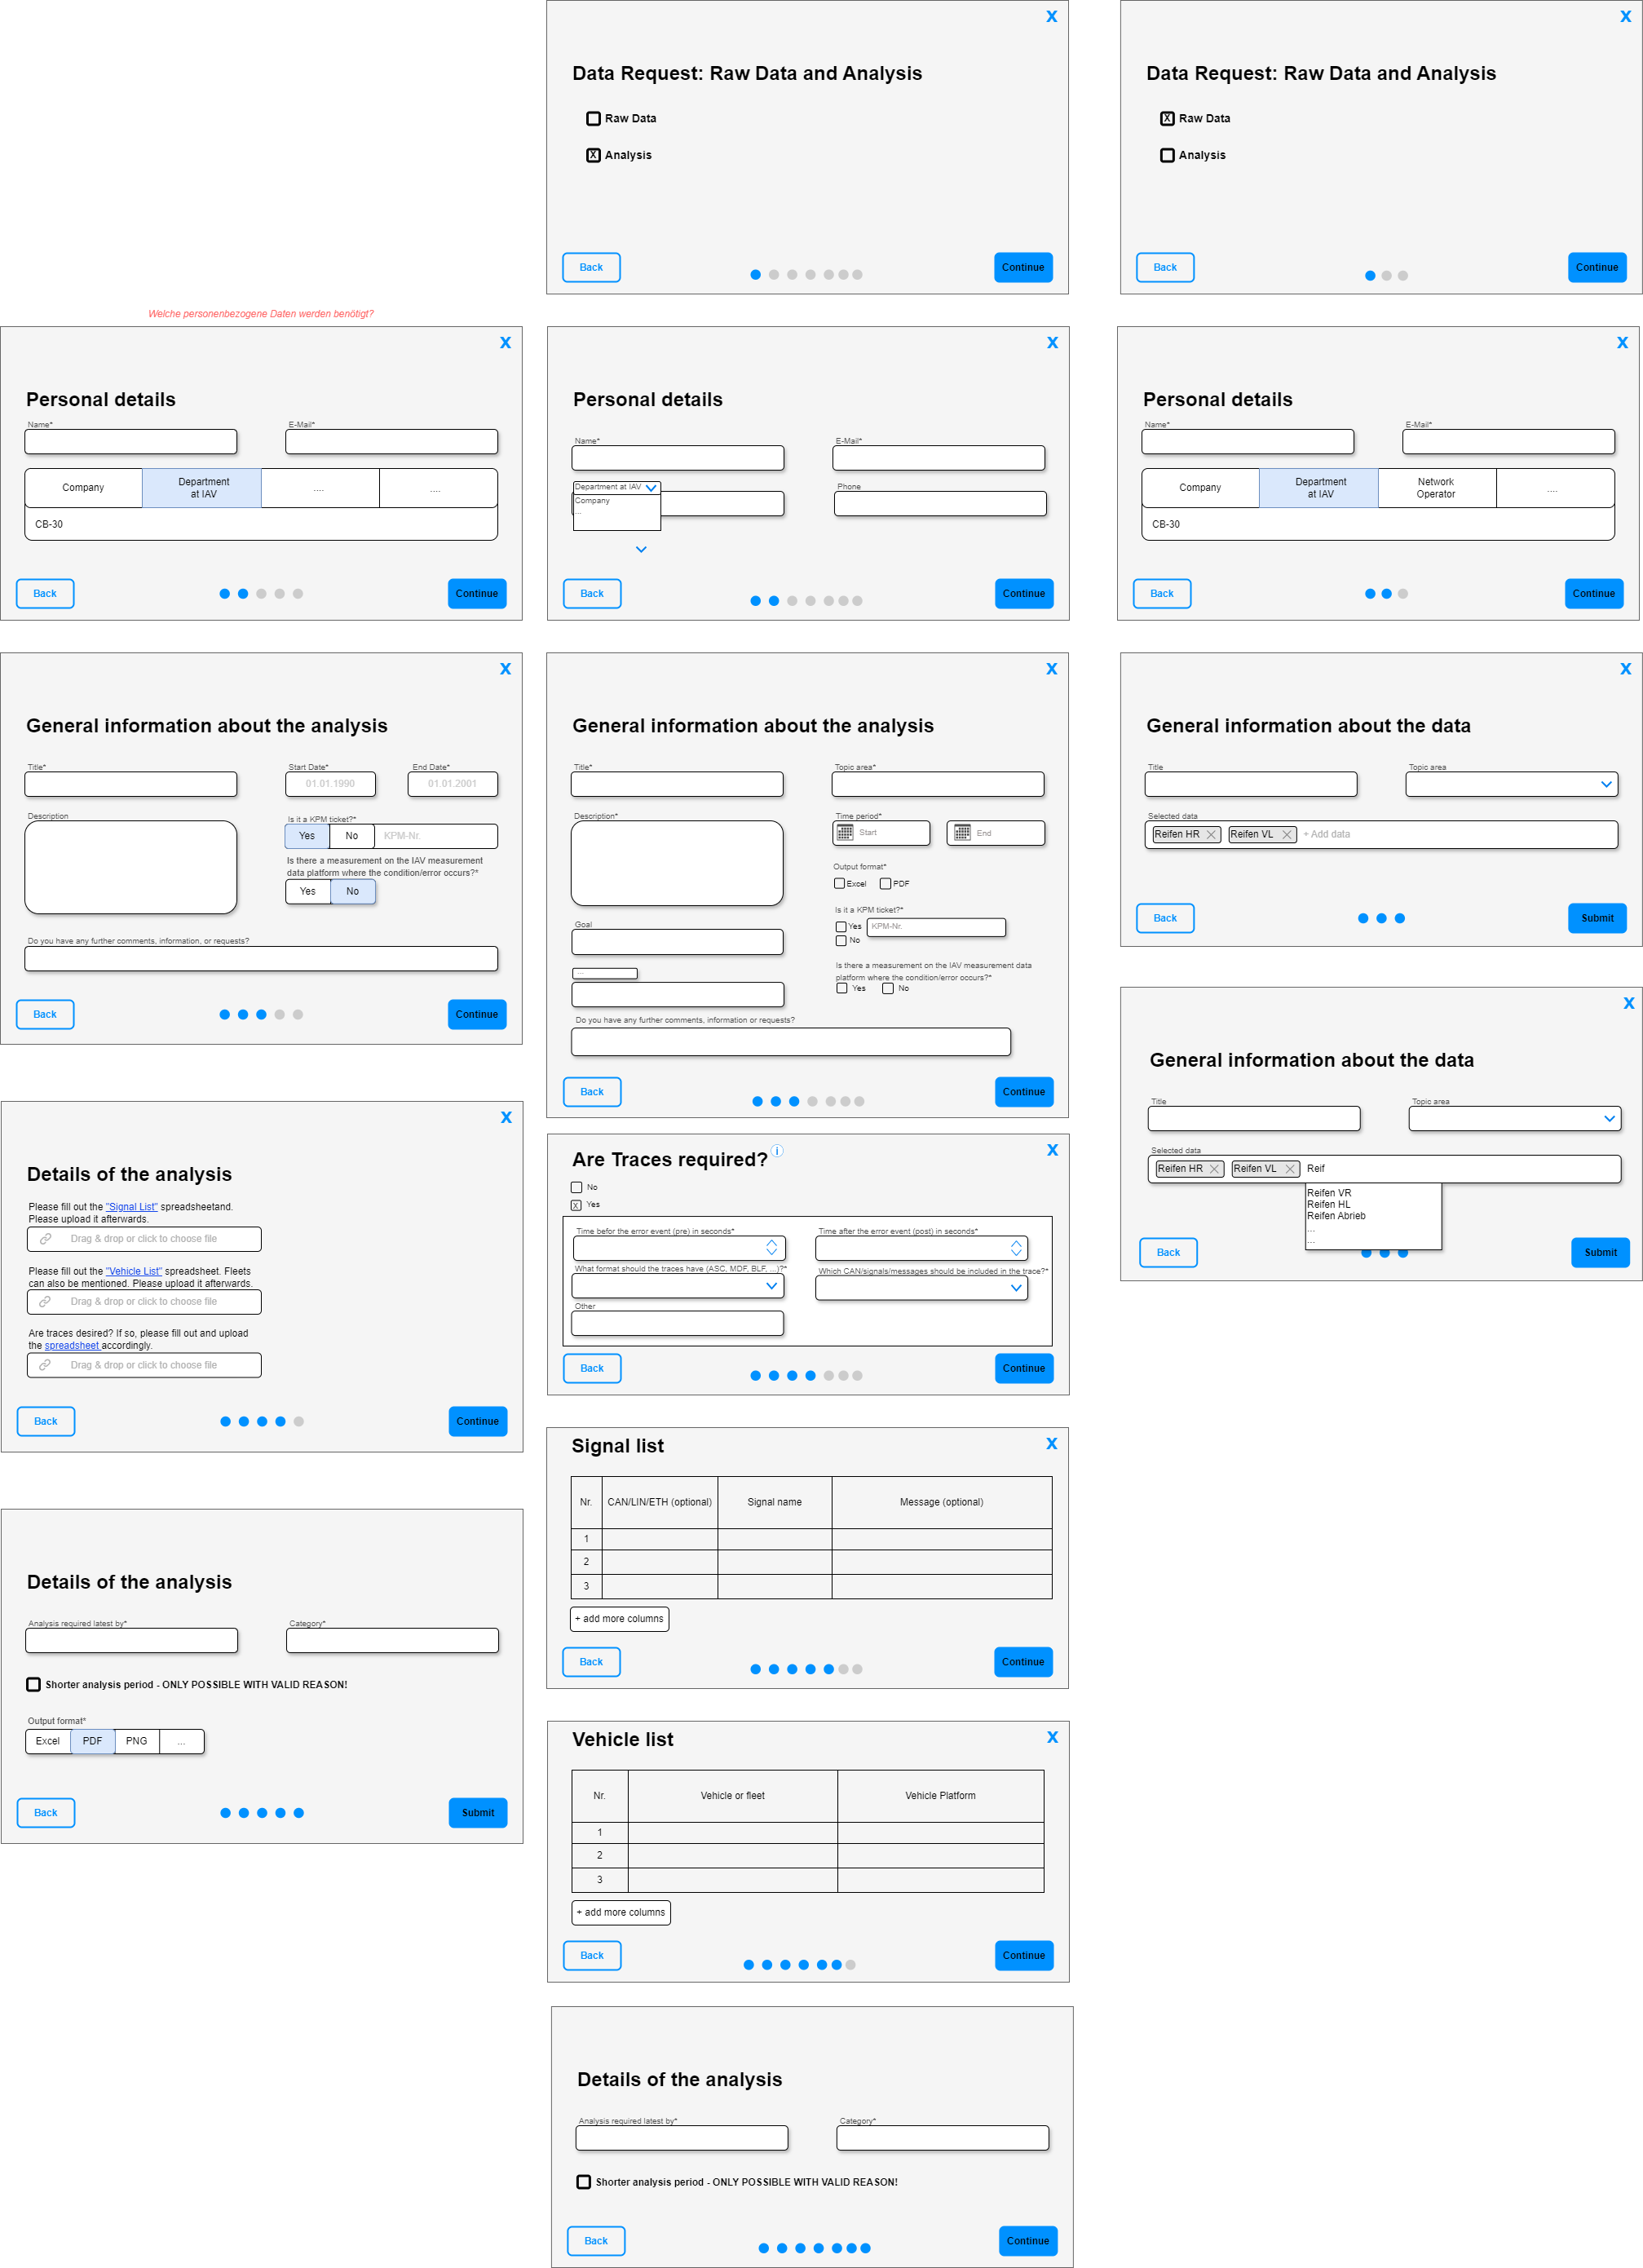
\includegraphics[scale=.2]{media/MockUps1.0}
    \caption{Mockup 1}
    \label{fig:MockUps1.0}
\end{figure}
\subsection*{Mockup 2}
Mit der zweiten Version, s. Abbildung \ref{fig:MockUps2.0}, wurde das Interface weiterentwickelt und dabei von der ursprünglichen BMW-Anlehnung gelöst. Es entstand ein individuelleres Design, das besser auf die spezifischen Anforderungen des Projekts zugeschnitten war. Dabei lag der Fokus auf einer verbesserten Benutzerführung und einer klareren Strukturierung der Formulare. Die Eingabefelder wurden optimiert, um eine bessere Lesbarkeit zu gewährleisten, und die Navigation wurde an den Workflow der Benutzer angepasst. Zusätzliche Hilfetexte und visuelle Hinweise führten den Benutzer durch den gesamten Anforderungsprozess. Diese Version stellte einen ersten großen Schritt in Richtung eines eigenständigen Tools dar.
\begin{figure}[H]
    \centering
    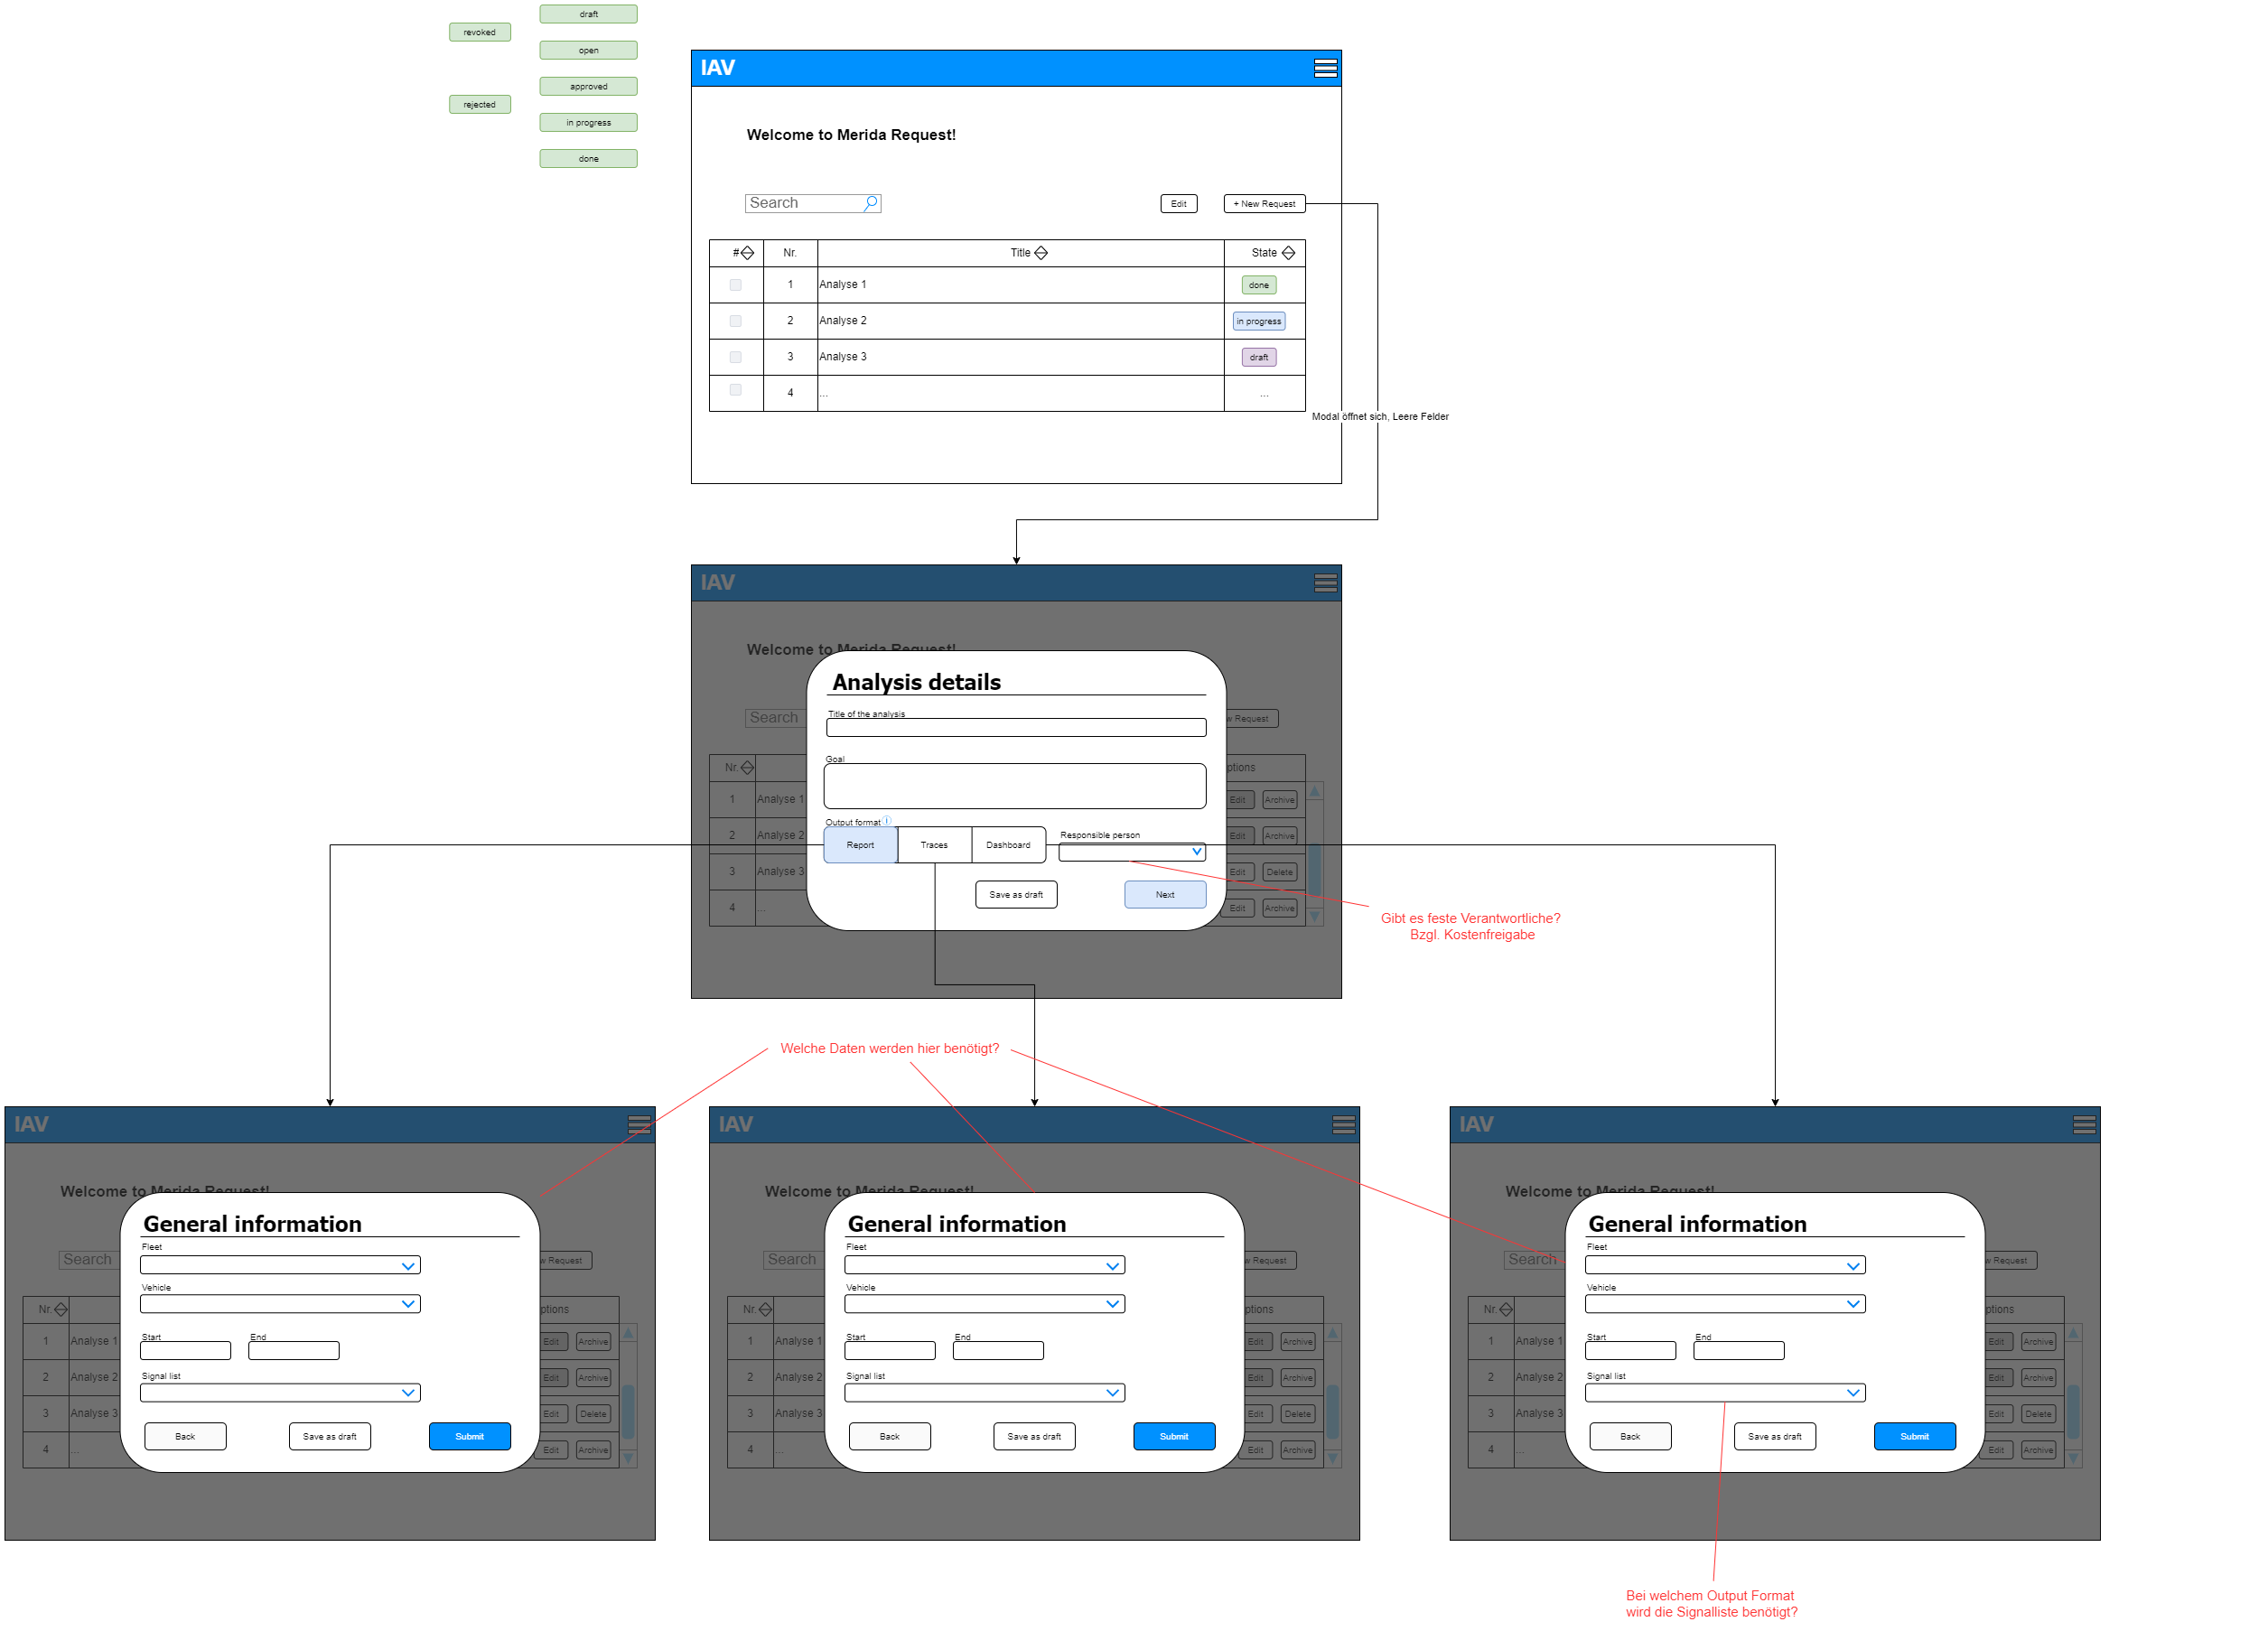
\includegraphics[scale=.2]{media/MockUps2.0}
    \caption{Mockup 2}
    \label{fig:MockUps2.0}
\end{figure}
\subsection*{Mockup 3 (Aktueller Stand)}
Das in der Abbildung \ref{fig:MockUps3.0} dargestellte Mockup repräsentiert den aktuellen Stand der Entwicklung und zeigt eine weiterentwickelte und verfeinerte Benutzeroberfläche. Hier liegt der Schwerpunkt auf dem Outputformat eines Dashboards und darauf, ein ausgereiftes und benutzerfreundliches System anzubieten, das sowohl funktional als auch optisch ansprechend ist.
\newline
Wichtige Änderungen in dieser Version:
\begin{itemize}
    \item Das Interface wirkt nun deutlich moderner und aufgeräumter. Es gibt eine klare Hierarchie in der Darstellung der Informationen, und die wichtigsten Optionen (wie die Auswahl des gewünschten Ausgabetyps) sind hervorgehoben.
    \item Die Benutzerführung wurde durch weitere Schritte verfeinert. Dazu gehören neue Kategorien für Diagrammtypen sowie eine präzisere Auswahloption für Flotten und Fahrzeuge. Die Auswahl erfolgt nun über eine Drag-and-Drop-Funktion, was die Bedienung vereinfacht und intuitiver gestaltet.
    \item Der Nutzer kann nun mehrere Diagramme im Stil eines Dashboards anlegen und konfigurieren. Am Ende des Prozesses erhält er eine zusammenfassende Übersicht über die erstellte Anfrage.
    \item Benutzer haben jetzt die Möglichkeit, Anfragen als Entwurf zu speichern und später weiterzubearbeiten. Diese Funktion erhöht die Effizienz und unterstützt eine flexible Arbeitsweise. 
\end{itemize}
\begin{figure}[H]
    \centering
    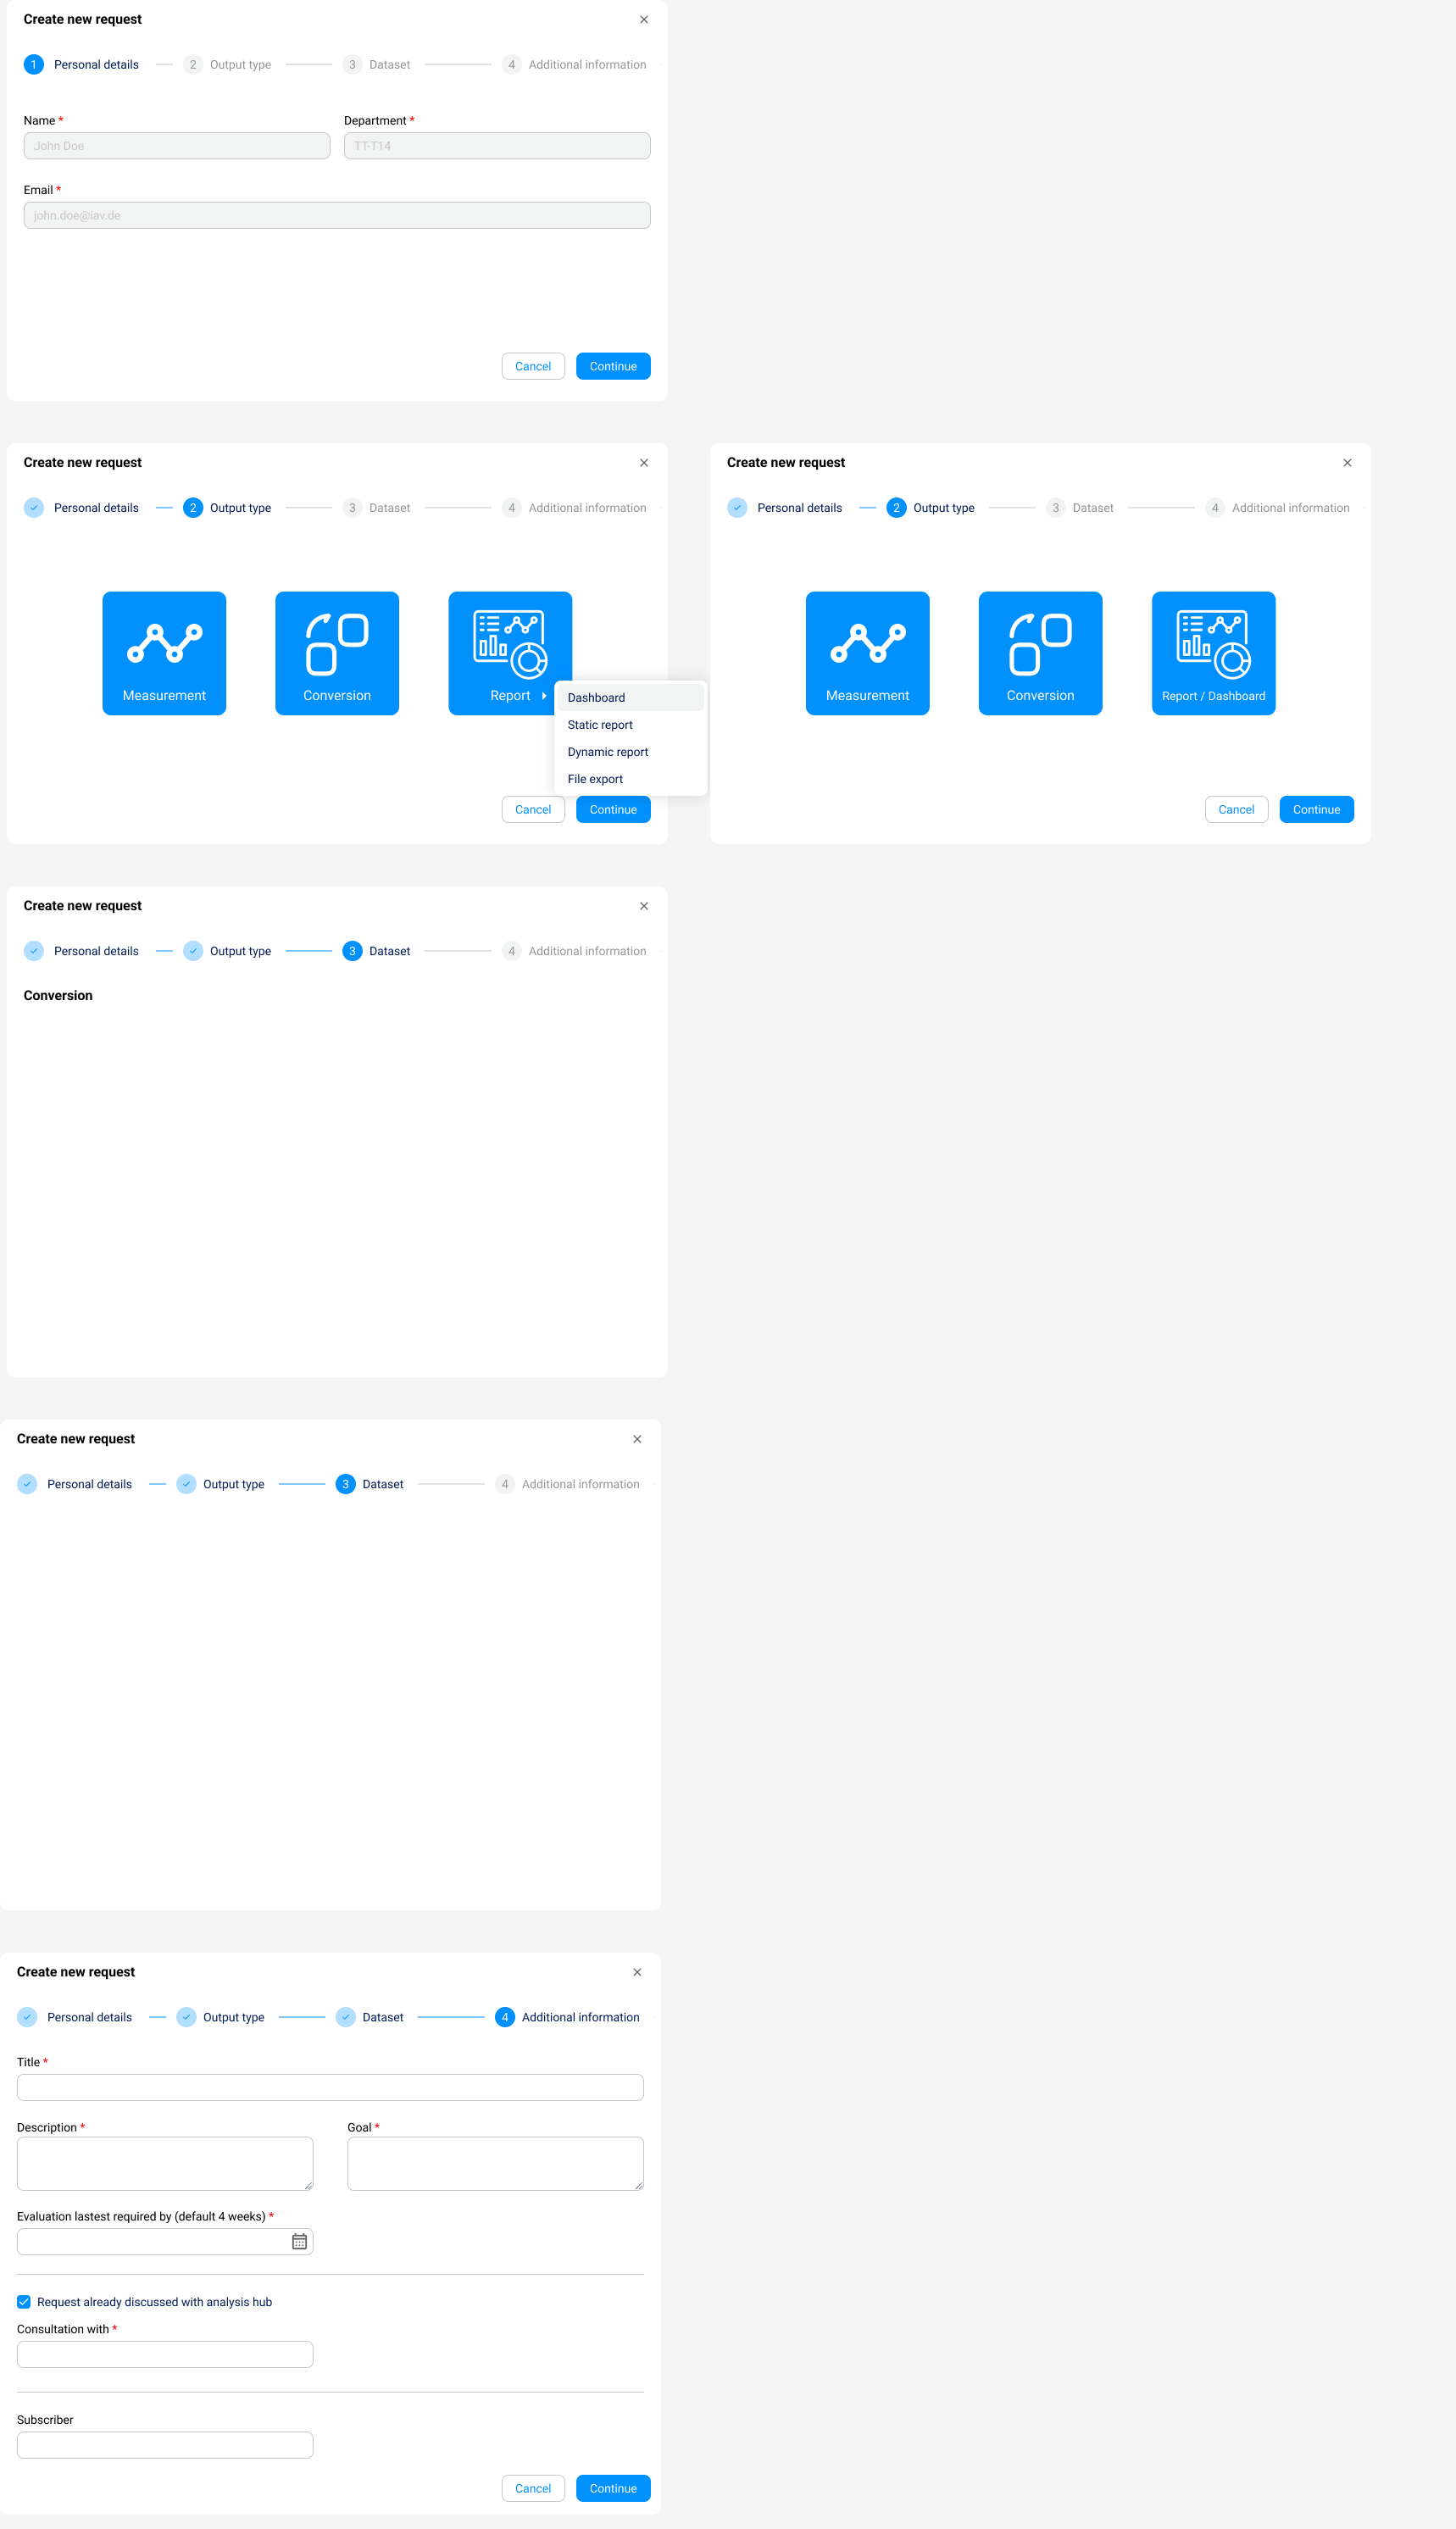
\includegraphics[scale=.25]{media/MockUps3.0}
    \caption{Mockup 3}
    \label{fig:MockUps3.0}
\end{figure}
Zusammenfassend lässt sich sagen, dass sich das IAV Merida Request Tool durch einen iterativen Entwicklungsprozess erheblich weiterentwickelt hat. Während Mockup 1 noch stark an bestehende Lösungen angelehnt war, strebte Mockup 2 bereits ein eigenständiges Design mit klareren Nutzerführungen an. Mit Mockup 3 erreicht das Tool nun ein hohes Maß an Benutzerfreundlichkeit, Flexibilität und Funktionalität, dass den Anforderungen der Benutzer in vollem Umfang gerecht wird.
\newpage
\section{Workflow}
Der dargestellte Workflow (s. Abbildung \ref{fig:Workflow}) beschreibt den vollständigen Ablauf eines Anfrageprozesses, der mehrere Phasen durchläuft, um eine effiziente und strukturierte Bearbeitung sicherzustellen. Dieser Prozess beginnt mit der Erstellung einer Anfrage und endet mit der finalen Analyse.
\subsection*{Entwurfsphase (Draft)}
Der Prozess beginnt mit der Erstellung der Anfrage. In dieser Phase bereitet der Antragsteller alle relevanten Informationen vor, die für die Anfrage notwendig sind. Die Anfrage wird jedoch noch nicht an die zuständigen Personen gesendet, sondern verbleibt als Entwurf. Hier kann der Antragsteller die Anfrage noch überarbeiten, Details hinzufügen oder Anpassungen vornehmen. Der Entwurfsstatus ermöglicht es, die Anfrage zu optimieren, bevor sie offiziell eingereicht wird. Sobald der Antragsteller alle notwendigen Informationen eingetragen hat und bereit ist, die Anfrage weiterzuleiten, wird diese in den nächsten Schritt überführt.
\subsection*{Offene Phase (Open)}
Sobald die Anfrage finalisiert ist, wird sie aus dem Entwurfsstatus versendet. In der Phase \texttt{Open} wird die Anfrage einer verantwortlichen Person zugewiesen, die anschließend die Bearbeitung übernimmt. Dieser Schritt ist entscheidend, da hierdurch die Verantwortung für den weiteren Verlauf eindeutig festgelegt wird.
\subsection*{In Bearbeitung (In Progress)}
In dieser Phase wird die Anfrage aktiv bearbeitet. Die verantwortliche Person prüft zunächst die Anfrage und den damit verbundenen Arbeitsaufwand. Ein wichtiger Entscheidungspunkt in diesem Abschnitt ist, ob es noch offene Fragen gibt, die mit dem Antragsteller geklärt werden müssen. Falls Fragen bestehen, wird der Antragsteller kontaktiert, um Unklarheiten zu beseitigen und gegebenenfalls zusätzliche Informationen anzufordern.
\newline
Sobald alle notwendigen Informationen vorliegen und alle Fragen geklärt sind, beginnt die Erstellung der Analyse. Diese Analyse kann je nach Anfrageumfang und -komplexität unterschiedlich viel Zeit in Anspruch nehmen. Die Analyse ist der Kern des Bearbeitungsprozesses, da hier die eigentliche Auswertung der angeforderten Daten oder Informationen stattfindet.
\newline
Während der Analysephase ist es weiterhin möglich, dass der Antragsteller oder die verantwortliche Person Rückfragen haben oder zusätzliche Details geklärt werden müssen. Es kann notwendig sein, dass eine enge Zusammenarbeit zwischen dem Analysten und dem Antragsteller erforderlich ist, um sicherzustellen, dass die Analyse den Erwartungen entspricht.
\subsection*{Abgelehnt/Zur{\"u}ckgezogen (Rejected/Revoked)}
Falls die Einigung zwischen dem Antragsteller und dem Analysten nicht erreicht wird, oder wenn während des Prozesses festgestellt wird, dass die Anfrage nicht weiter verfolgt werden kann, wird die Anfrage in den Status \texttt{Rejected} oder \texttt{Revoked} versetzt. Dieser Status beendet den Anfrageprozess vorzeitig. Gründe für diesen Abbruch könnten unklare Anforderungen, nicht erfüllbare Bedingungen oder andere Hindernisse sein, die den Abschluss der Anfrage verhindern.
\subsection*{Abschlussphase (Done)}
Sobald die Analyse abgeschlossen und alle offenen Punkte geklärt sind, wird das Ergebnis an den Antragsteller übermittelt. Mit der Zusendung der Analyse endet der Prozess, und der Status der Anfrage wird auf \texttt{Done} gesetzt.
\newline
\begin{figure}[H]
    \centering
    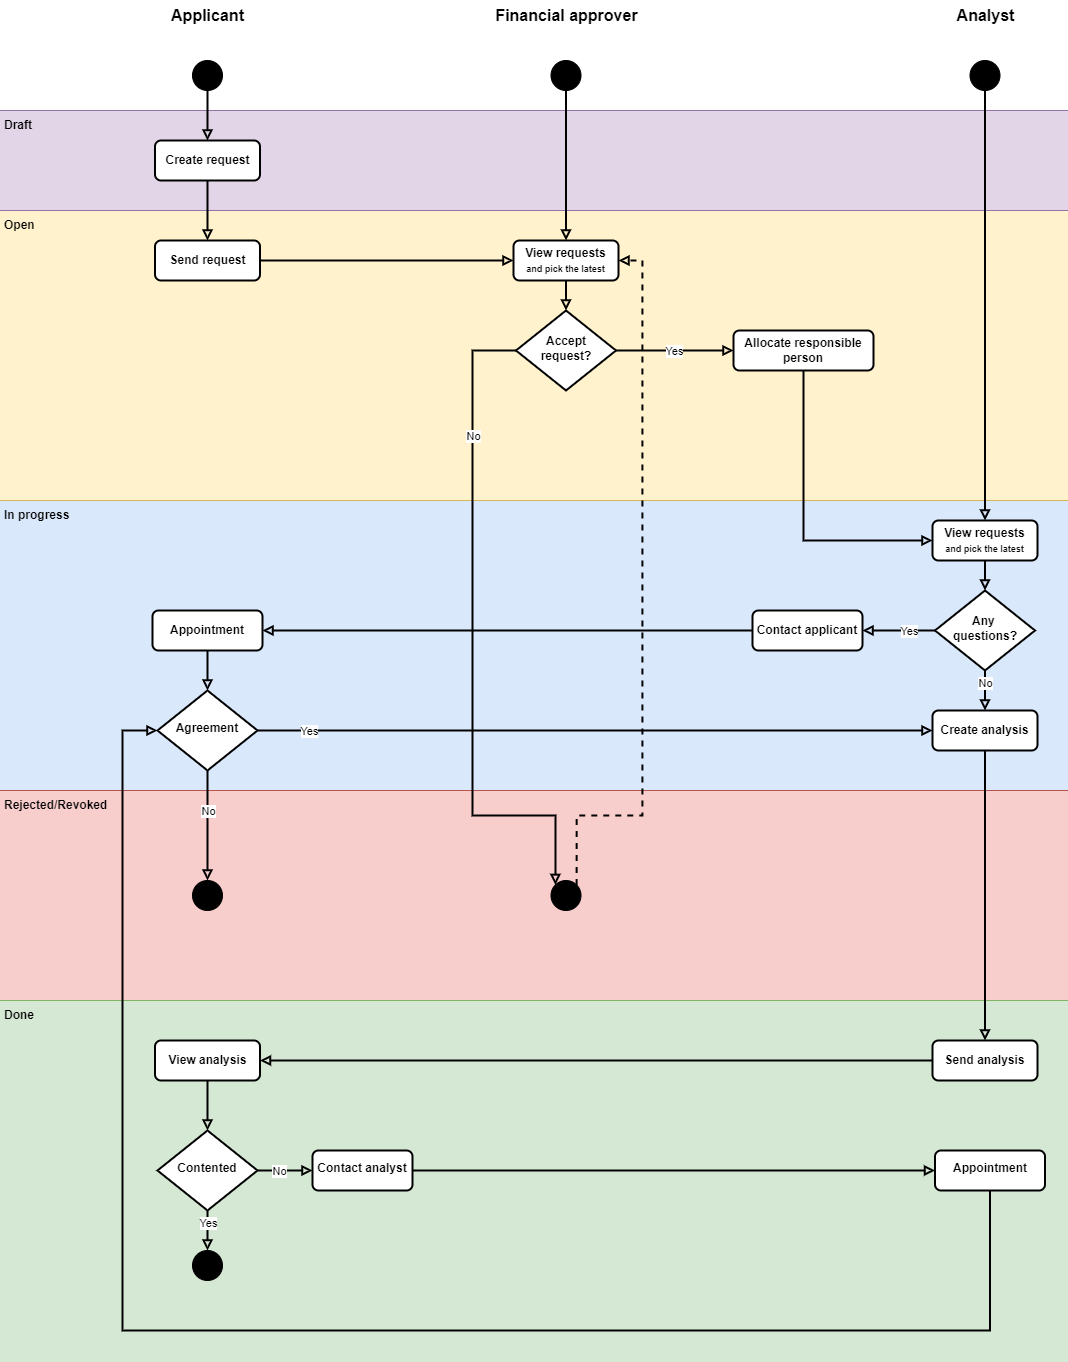
\includegraphics[scale=.4]{media/Workflow}
    \caption{Workflow}
    \label{fig:Workflow}
\end{figure}
\newpage
\section{Architektur}
Die Architektur der entwickelten Softwarelösung basiert auf modernen, skalierbaren und wartbaren Technologien, die auf die spezifischen Anforderungen des Projekts abgestimmt sind. Das System besteht aus drei Hauptkomponenten: dem Backend, das mit NestJS entwickelt wurde, dem Frontend das auf React basiert und einer relationalen Datenbank, die durch PostgreSQL unterstützt wird. Um eine flexible und isolierte Datenbankumgebung zu gewährleisten wird PostgreSQL über Docker containerisiert, was eine einfache Bereitstellung und Verwaltung verschiedener Entwicklungs- und Produktionsumgebungen ermöglicht (s. Abbildung \ref{fig:Architekturdiagramm}). 
\newline
\newline
Das Frontend wird im Rahmen einer Microfrontend-Architektur entwickelt, bei der das React-basierte Interface als eine von mehreren Anwendungen innerhalb eines größeren Systems integriert wird. Diese Architektur ermöglicht es, unterschiedliche Frontends, die mit verschiedenen Technologien entwickelt wurden, nahtlos zu kombinieren und gleichzeitig eine modulare Struktur beizubehalten. Jede Anwendung (Microfrontend) ist in sich eigenständig, kann aber über standardisierte Schnittstellen miteinander kommunizieren. Auf diese Weise können unterschiedliche Technologien und Teams gleichzeitig an verschiedenen Microfrontends arbeiten, was die Flexibilität und Skalierbarkeit des Systems erhöht.
\newline
\newline
NestJS bietet eine robuste und strukturierte Grundlage für die Backend-Entwicklung. Die serviceorientierte Architektur in Kombination mit der \ac{MVC}-Ansatz, wie ihn NestJS vorgibt, stellt sicher, dass die Geschäftslogik effizient isoliert und die verschiedenen Komponenten voneinander getrennt sind.
\newline
Die Kommunikation zwischen den einzelnen Komponenten erfolgt über klar definierte Schnittstellen und standardisierte Protokolle. Das Frontend interagiert mit dem Backend über HTTP-APIs unter Verwendung von RESTful-Endpunkten. Diese APIs ermöglichen eine effiziente und flexible Kommunikation zwischen Benutzeroberfläche und Serverlogik, wobei JSON als Standardformat für die Datenübertragung verwendet wird.
\newline
Das NestJS-Backend übernimmt die zentrale Rolle in der Geschäftslogik des Systems. Es stellt den Datenzugriff auf die PostgreSQL-Datenbank bereit und kümmert sich um die Verarbeitung der Daten. Die Datenbank wird über ein \ac{ORM} angesprochen, in diesem Fall ein TypeORM, was eine effiziente und strukturierte Kommunikation zwischen den Anwendungen und der relationalen Datenbank ermöglicht. Zusätzlich gibt es die Schnittstelle zum IAV Merida Hub, die den Import von Flotten und Fahrzeugdaten in die lokale Datenbank ermöglicht. Durch die asynchrone Kommunikation über API-Aufrufe bleibt die Datenbasis stets aktuell und wird in Echtzeit mit dem IAV Merida Hub synchronisiert.
Mittels der folgenden Abbildung wird verdeutlicht, wie die einzelnen Schichten miteinander kommunizieren.
\begin{figure}[H]
    \centering
    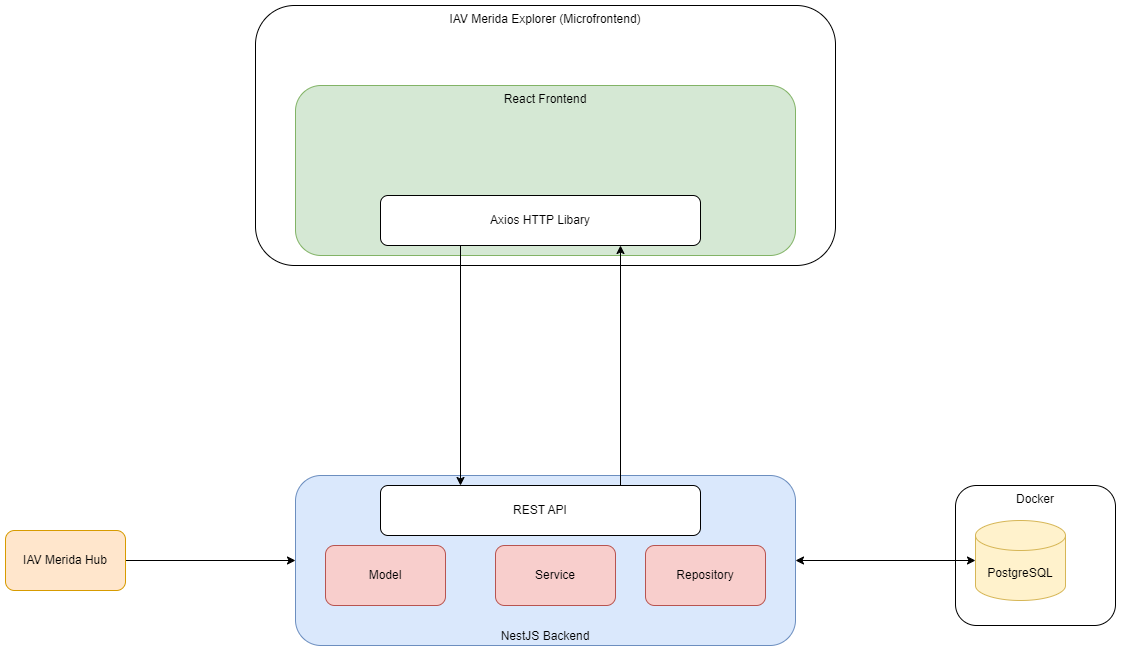
\includegraphics[scale=.4]{media/Architekturdiagramm}
    \caption{Architekturdiagramm}
    \label{fig:Architekturdiagramm}
\end{figure}
Ein zusätzliches Komponentendiagramm (s. Abbildung \ref{fig:Komponentendiagramm}) zeigt die Schnittstellen zwischen Backend, Frontend und Datenbank sowie die Verbindung zu externen Systemen. Es verdeutlicht, wie das Backend die im IAV Merida Hub gespeicherten Flotten- und Fahrzeugdaten abruft, sodass Nutzer im Frontend Flotten und – optional – Fahrzeuge auswählen kann, für die sie Messdaten und Analysen einsehen möchten.
\newline
Neben dem Merida Request-Modul bietet der IAV Merida Explorer aktuell weitere Module. Dazu gehören der Merida Transmitter für den gesicherten und automatisierten Upload von Messdaten aus verschiedenen Quellen, der Merida Signals Web für einen direkten Einblick in die verfügbaren Messdaten sowie der Merida Finder, der durch eine spezielle Suchmaske komplexe Suchanfragen über alle Messungen hinweg ermöglicht. Das Merida Dashboard visualisiert schließlich verschiedene Analysen der gesammelten Daten.
\newline
Für die Zukunft ist die Integration einer Schnittstelle zu Confluence geplant, um den Analysten eine erleichterte Dokumentation einzelner Anfragen zu ermöglichen.
\newline
Außerdem ist noch unklar, wie die Verwaltung der Daten- und Analyseanfragen erfolgen soll. Im Gespräch ist derzeit Jira, das als Ticketsystem für Anfragen dienen könnte, um die Zuweisung an Analysten zu erleichtern und einen besseren Überblick über die offenen Aufgaben zu gewährleisten. Allerdings gab es in der Vergangenheit einige Schwierigkeiten mit Jira, weshalb noch zu prüfen ist, ob Jira tatsächlich eine geeignete Lösung darstellt oder ob eine Eigenimplementierung sinnvoller wäre.
\begin{figure}[H]
    \centering
    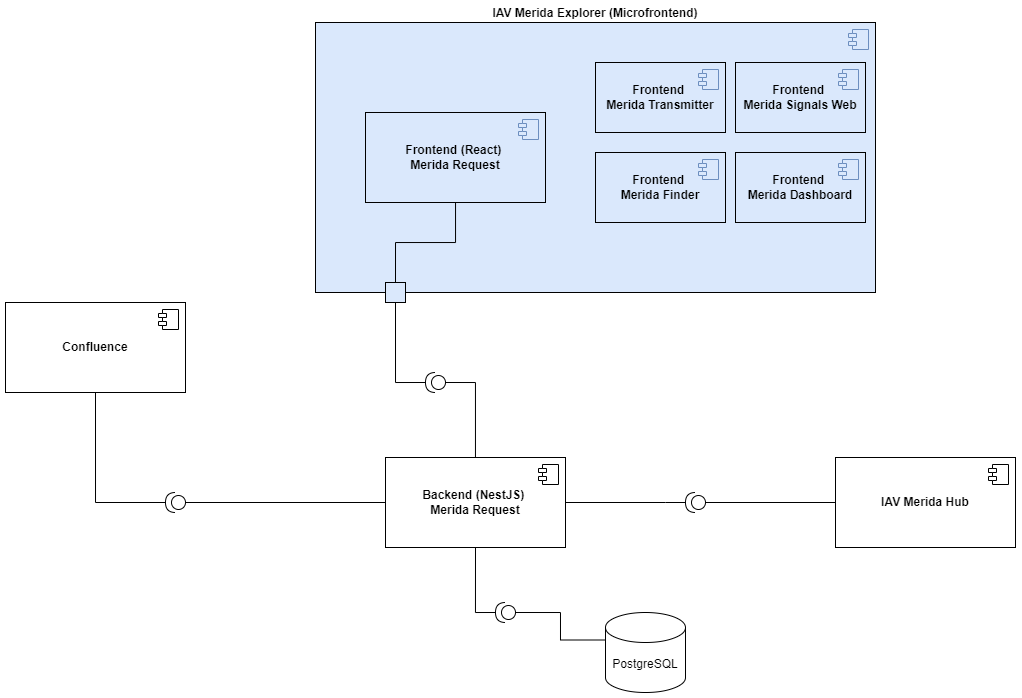
\includegraphics[scale=.4]{media/Komponentendiagramm}
    \caption{Komponentendiagramm}
    \label{fig:Komponentendiagramm}
\end{figure}
\label{chap:kapitel5}

%\chapter{Einzelne Aspekte der Implementierung}
In diesem Kapitel werden die Hauptfunktionen und Module des Backends erläutert. Dabei werden die zugrunde liegende Architektur, der Datenfluss und die Interaktion der einzelnen Komponenten detailliert beschrieben. Auch Herausforderungen, die im Verlauf der Implementierung aufgetreten sind, werden thematisiert, um die Lösungsansätze und Entscheidungsprozesse nachvollziehbar darzustellen.
\newline
\newline
Für das Projekt wurde eine service-orientierte \ac{MVC}-Architektur gewählt, die eine klare Trennung der Verantwortlichkeiten ermöglicht und eine hohe Modularität aufweist. Diese Architektur bietet den Vorteil, dass die Codebasis leicht erweiterbar bleibt, was besonders wichtig war, da die Anforderungen im Verlauf des Projekts mehrfach angepasst wurden.
\subsubsection*{Aufbau und Funktion der einzelnen Komponenten}
Jede Entität verfügt über einen eigenen Controller, der die Anfragen des Clients verarbeitet und die Schnittstelle zur Außenwelt darstellt. Der Controller übernimmt die Kommunikation und Steuerung, indem er eingehende Anfragen validiert, die zuständigen Services aufruft und die Antworten in einem geeigneten Format an den Client zurückgibt. So bleibt die Controller-Schicht schlank und frei von Geschäftslogik, da diese vollständig in die Service-Schicht ausgelagert ist.
\newline
In der Service-Schicht wird die Geschäftslogik gekapselt und die Interaktion mit der Datenbank verwaltet. Hier werden alle geschäftsrelevanten Operationen implementiert, wie etwa das Verarbeiten von CRUD-Operationen (Create, Read, Update, Delete) für die einzelnen Entitäten. Durch die zentrale Bündelung der Geschäftslogik in den Services bleibt diese unabhängig von der Controller-Schicht und kann für verschiedene Anwendungsfälle wiederverwendet werden.
\newline
Die Entitäten definieren die Struktur der Daten und die Beziehungen zwischen den Objekten, die in der PostgreSQL-Datenbank gespeichert werden. Mithilfe von TypeORM, einem objekt-relationalen Mapper (ORM), werden die Entitäten automatisch mit der Datenbank synchronisiert. TypeORM abstrahiert dabei die Datenbankoperationen und ermöglicht so eine vereinfachte und fehlerfreie Datenverwaltung. Diese Abstraktion erleichtert die Wartung und Weiterentwicklung der Datenstruktur, da Änderungen in der Datenbank über das ORM gesteuert und in den Entitäten abgebildet werden können.
\subsubsection*{API-Integration zur Datenabfrage externer Ressourcen}
Eine wesentliche Anforderung im Projekt war die Anbindung an das Merida Hub Playground, um Flotten- und Fahrzeugdaten in das Anfragetool zu integrieren und den Benutzern zur Verfügung zu stellen. Hierfür wurde eine API-basierte Kommunikation entwickelt, die Daten aus externen Quellen abruft und in das System importiert.
\newline
Zur Echtzeitabfrage der Daten von Flotten und Fahrzeugen wurden Methoden implementiert, die über HTTP-Requests auf die Endpunkte der Merida-Hub-API zugreifen. Diese Methoden greifen auf Authentifizierungsdaten und eine gesicherte HTTPS-Verbindung zurück, um den API-Zugriff sicherzustellen.
\newline
Ein Beispiel für die Methode zur Abfrage von Fahrzeugdaten einer spezifischen Flotte sieht wie folgt aus:
\lstset{ % Konfiguration für das Aussehen des Codes
    language=JavaScript, % Programmiersprache
    basicstyle=\ttfamily\small, % Schriftstil und -größe
    keywordstyle=\color{blue}\bfseries, % Stil für Schlüsselwörter
    commentstyle=\color{gray}, % Stil für Kommentare
    stringstyle=\color{purple}, % Stil für Strings
    numbers=left, % Zeilennummerierung links
    numberstyle=\tiny, % Stil der Zeilennummern
    stepnumber=1,
    breaklines=true, % Zeilenumbruch
    frame=single, % Rahmen um den Code
    xleftmargin=15pt, % Linker Rand
}

\begin{lstlisting}
    // Fetch fleets from external API
    async fetchFleetsFromApi(): Promise<any> {
      const endpoint = 'https://m3-frontend-m3-playground.c1.k8s.iavgroup.local/api/lists/fleets';
   
      try {
        const response = await lastValueFrom(
          this.httpService.get(endpoint, {
            httpsAgent: this.httpsAgent,
            auth: {
              username: '******',
              password: '*****',
            },
          })
        );
   
        if (Array.isArray(response.data.data)) {
          // Transforme data
          const transformedData = response.data.data.map(fleet => ({
            fleet_id: fleet.id,
            fleet_name: fleet.name,
          }));
          return transformedData;
        } else {
          throw new Error('API response data is not an array');
        }
      } catch (error) {
        console.error('Error fetching fleets from API:', error);
        throw new HttpException('Failed to fetch fleets from API', 500);
      }
    }
\end{lstlisting}
Diese Methode ermöglicht es, die Fahrzeugdaten strukturiert zu verarbeiten und die relevanten Informationen wie Fahrzeug- und Flotten-IDs und Namen in einem formatgerechten Objekt abzubilden. Dadurch wird sichergestellt, dass die Daten korrekt und übersichtlich im Anfragetool angezeigt werden können.
\subsubsection*{Herausforderungen und Lösungsansätze bei der API Integration}
Bei der API-Integration traten mehrere Herausforderungen auf, wie die Authentifizierung für den API-Zugriff und das Management von Datenformaten, da es am Anfang Probleme beim Abrufen der Daten im Frontend gab, mussten die Daten in das richtige Format gebracht werden. Diese Herausforderungen wurden durch folgende Maßnahmen gelöst:
\begin{itemize}
    \item Sichere HTTPS-Verbindungen und Authentifizierung über httpsAgent, um die Integrität der Datenübertragung sicherzustellen.
    \item Transformation der abgerufenen Daten, wie im obigen Code gezeigt, um Informationen in dem entsprechende Format bereitzustellen.
\end{itemize}
\subsubsection*{Entscheidungsgründe für die Architektur}
Die Entscheidung für die service-orientierte MVC-Architektur basiert auf mehreren folgenden Faktoren:
\begin{itemize}
    \item Klare Trennung der Verantwortlichkeiten: Die Aufteilung in Controller, Service und Entitäten stellt sicher, dass jede Funktionalität in ihrem eigenen Bereich implementiert wird, was die Übersichtlichkeit und Wartbarkeit des Codes erhöht.
    \item Erweiterbarkeit: Durch die lose Kopplung zwischen den Schichten lassen sich neue Funktionen leicht hinzufügen, ohne dass bestehende Komponenten stark verändert werden müssen.
    \item Flexibilität bei unklaren Anforderungen: Da sich die Anforderungen im Laufe des Projekts mehrfach geändert haben, ermöglichte die modulare Struktur eine schnelle Anpassung und Erweiterung der Anwendung.
    \item Wiederverwendbarkeit der Geschäftslogik: Da die Geschäftslogik zentral in der Service-Schicht angesiedelt ist, können die Services von verschiedenen Controllern aufgerufen und flexibel für unterschiedliche Endpunkte genutzt werden.
\end{itemize}
\subsubsection*{Interaktion der Module und Datenfluss}
Der Datenfluss innerhalb der Anwendung folgt einem klaren Ablauf. Die Anfragen des Clients werden vom Controller empfangen und an den entsprechenden Service weitergeleitet. Im Service wird dann die Logik zur Bearbeitung der Anfrage ausgeführt. Bei Bedarf werden Datenbankabfragen initiiert, um Daten abzurufen oder zu aktualisieren. Die Antwort wird anschließend wieder an den Controller zurückgegeben und in einem geeigneten Format an den Client gesendet. Diese Struktur fördert die Nachvollziehbarkeit der Datenflüsse und vereinfacht die Fehlersuche und Wartung.
\newline
Insgesamt erlaubt diese Architektur eine strukturierte Entwicklung der Hauptfunktionen und Module und stellt sicher, dass die Anwendung flexibel bleibt. Die Trennung der Logik in die Module gewährleistet zudem, dass die Implementierung leicht anpassbar und wartbar ist, was für die Erweiterung und die Anpassungsfähigkeit des Projekts entscheidend ist.
\label{chap:kapitel6}

\chapter{Zusammenfassung und Ausblick}

\section{Zusammenfassung}

\section{Ausblick}


% ***************************** BIBLIOGRAPHY *******************************
\baselineskip=14pt
\clearpage
\phantomsection
\addcontentsline{toc}{chapter}{\protect\numberline{}\bibname}
\bibliography{bib/thesis}

% ******************************* APPENDIX *********************************
\appendix
\chapter{Anhang A}
\label{chap:anhang_a}





% ***************************** BACK MATTER ********************************
%\thispagestyle{empty}

%\addcontentsline{toc}{chapter}{\protect\numberline{}Eidesstattliche Erklärung}
%\section*{Erklärung}
\vspace*{0.5cm}
\noindent
Hiermit versichere ich, dass ich die vorliegende Arbeit selbstständig verfasst und keine anderen als die angegebenen Quellen und Hilfsmittel benutzt habe. Ich versichere, dass ich alle wörtlich oder sinngemäß aus anderen Werken übernommenen Aussagen als solche gekennzeichnet habe. Dies gilt explizit auch für die Verwendung von text- oder codegenerierenden KI-Werkzeugen.

Die eingereichte Arbeit ist weder vollständig noch in wesentlichen Teilen Gegenstand eines anderen Prüfungsverfahrens gewesen.

Ich habe zur Kenntnis genommen, dass die Arbeit einer elektronischen Plagiatsprüfung unterzogen werden kann.

\vspace{3cm}
\toponym, den \today

\end{document}
